\chapter{Le Grand collisionneur de hadrons (LHC)}
\renewcommand\chapterillustration{LHC/lhc}
\ThisULCornerWallPaper{1}{\chapterillustration}
\minitoc
\lettrine[lines=4, slope=-0.5em]{C}{e} chapitre décrit le complexe des accélérateurs du CERN\footnote{Organisation Européenne pour le Recherche Nucléaire (Laboratoire européen de physique des particules)} qui permet d'accélérer les particules, afin d'avoir un faisceau de particules avec une énergie suffisante pour être injecté dans le Grand Collisionneur de Hadrons (LHC\footnote{Large Hadron Collider}) et atteindre une énergie finale de $7$ TeV. Cette description bien que succincte est nécessaire car de nombreux résultats obtenus durant cette thèse ont nécessité l'utilisation d'accélérateurs de ce complexe. Une description du LHC est également donnée, car ses performances présentes et futures déterminent les choix technologiques des détecteurs utilisant son faisceau.

\section{Le complexe d'accélérateurs du CERN}

Le complexe d'accélération (\ref{complexe}) du CERN est une série de machines qui délivrent des faisceaux de particules d'énergies de plus en plus élevées. Chaque machine accélère les faisceaux et les injecte dans la machine suivante. Le dernier accélérateur du complexe est le LHC.

Le programme de ce dernier est surtout basé sur des collisions protons-protons. Cependant chaque année, environ un mois est consacré aux collisions d'ions lourds (plomb-plomb) ou (proton-plomb) afin d'étudier notamment le plasma de quarks et gluons, l'une des phases de l'Univers peu après le Big Bang. 

Dans le cas de ces collisions, la chaine d'accélération est constituée du Linear Accelerator 3 (LINAC 3), du Low Energy Ion Ring (LEIR) utilisé pour le stockage des ions et leur refroidissement. La chaine d'accélération est ensuite identique à celle pour les collisions proton-proton.

\begin{minipagewithmarginpars}[h]{\textwidth}
  	\centering
	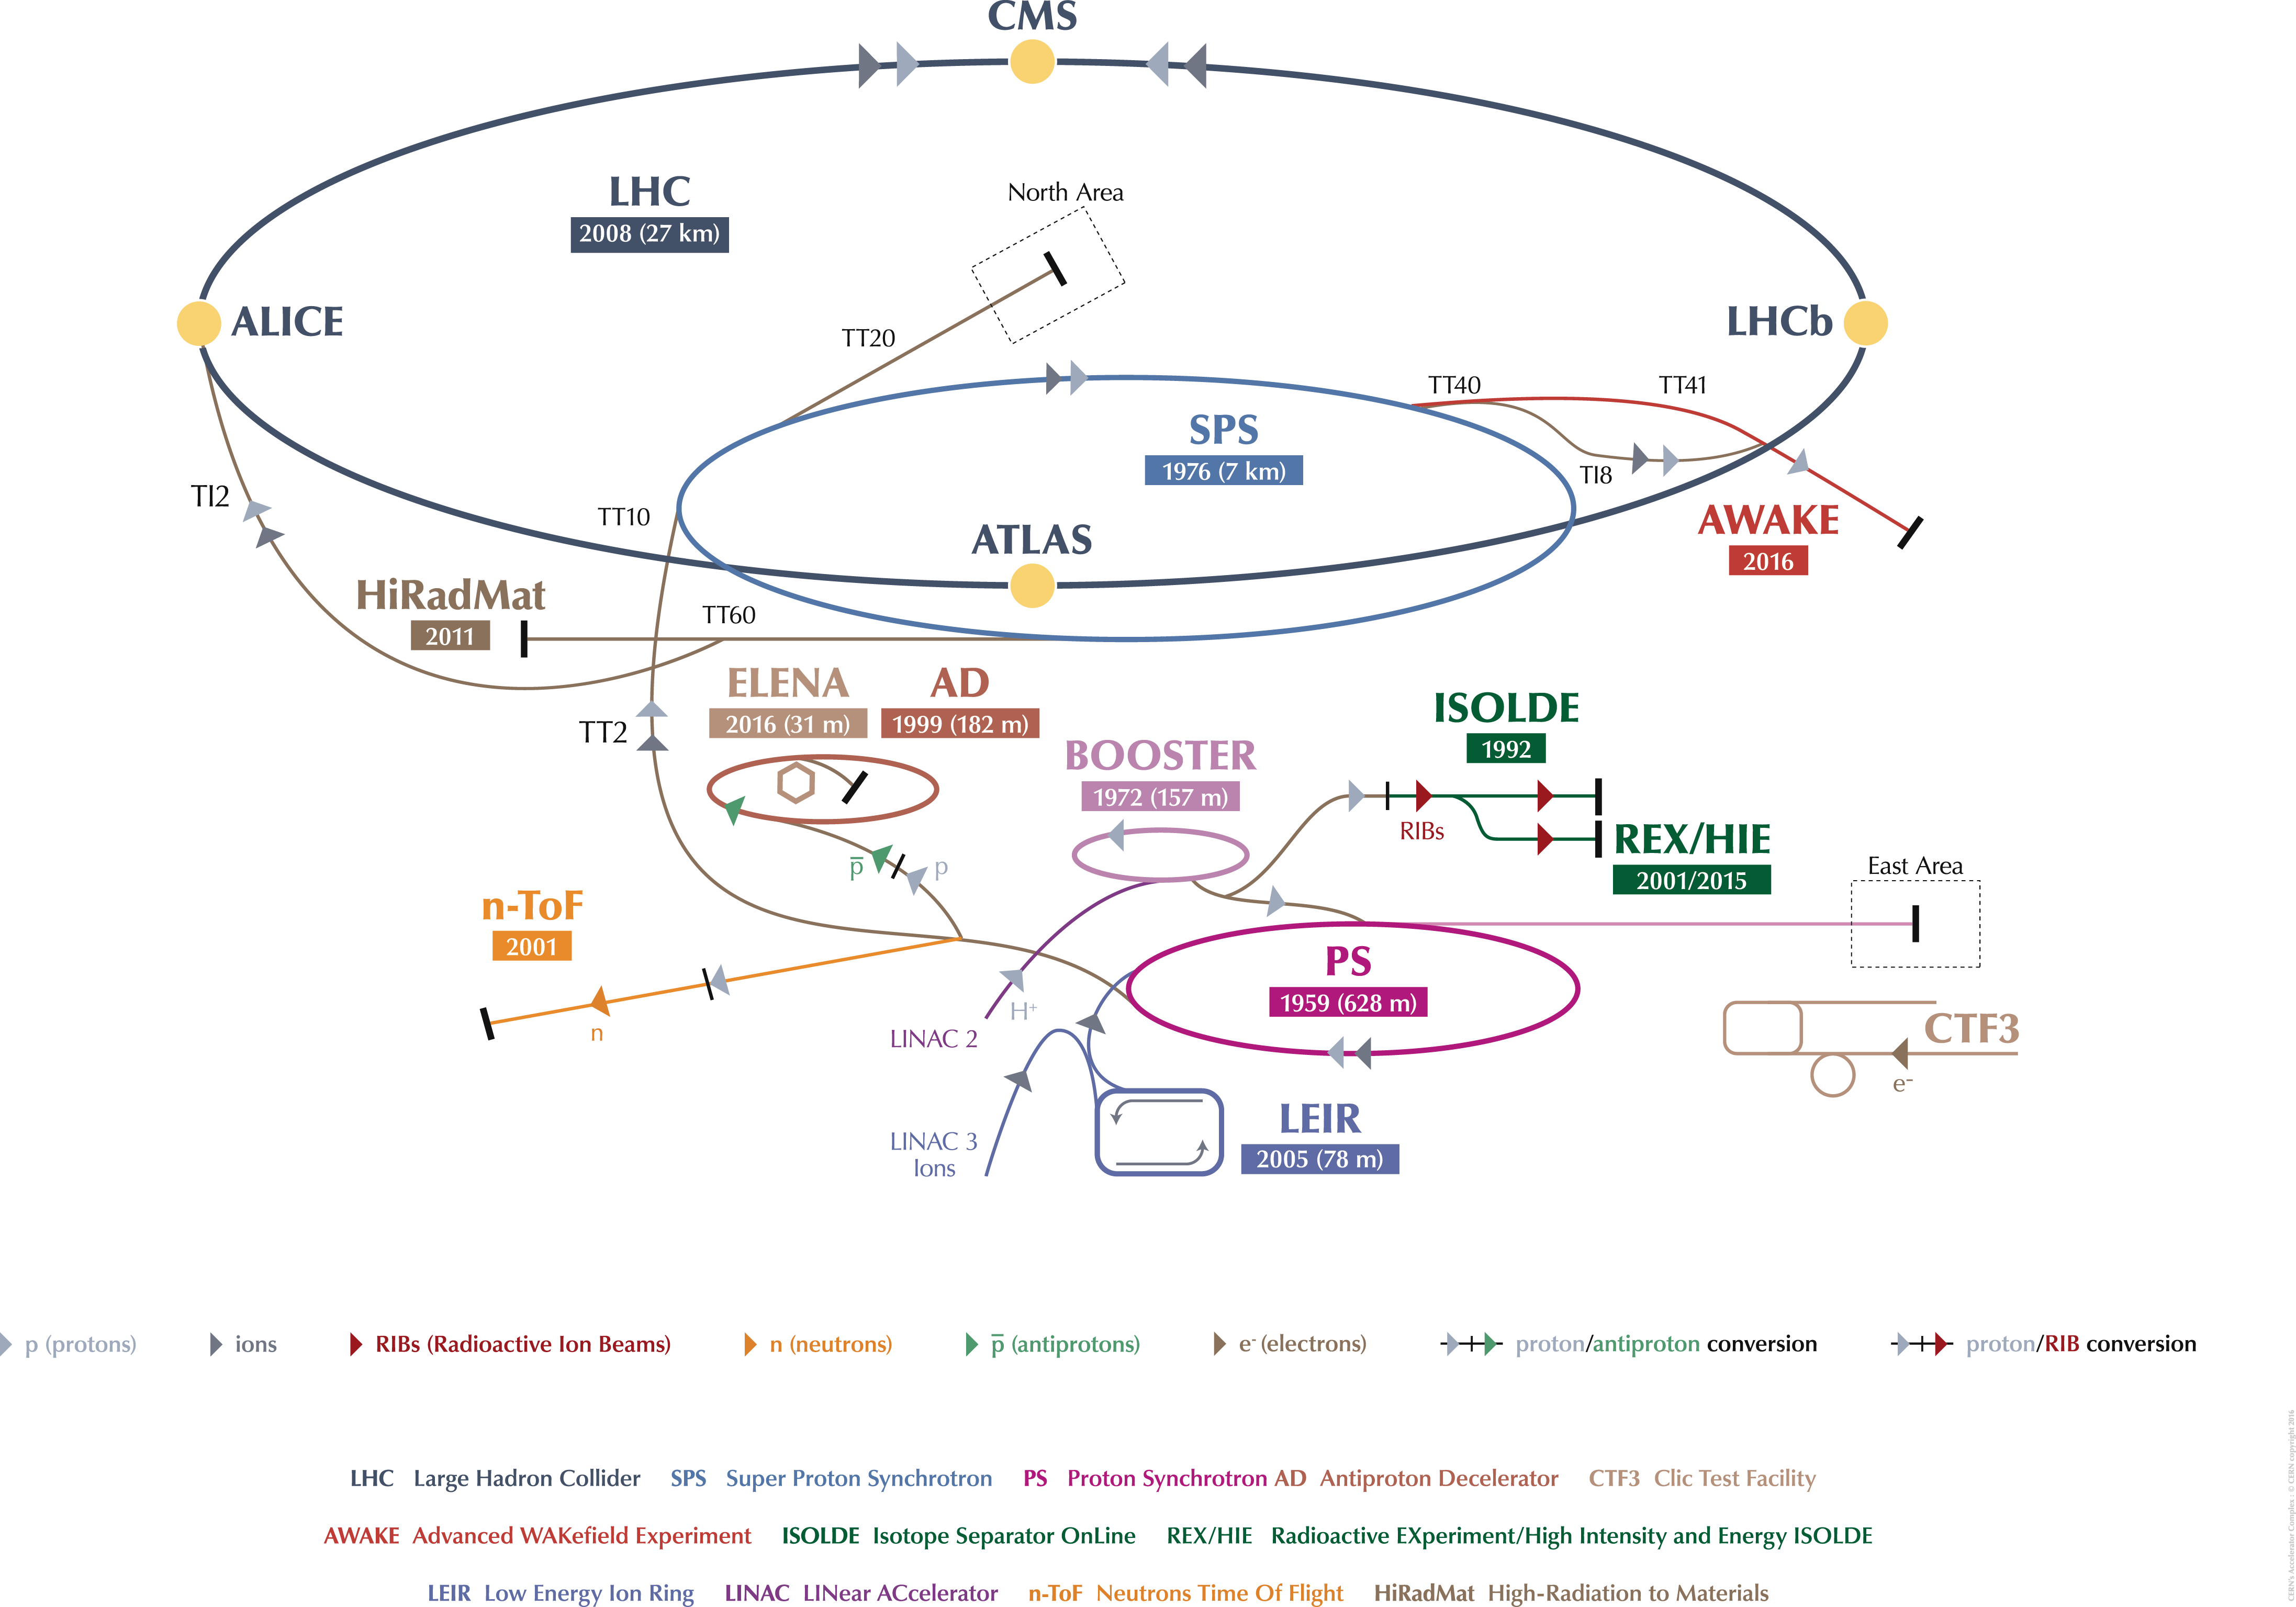
\includegraphics[scale=0.40]{LHC/complexe.png}
  	\captionof{figure}{Schéma du complexe d'accélération du CERN. La chaine d'injection du LHC est constituée du Linac 2, du Booster, du PS et du SPS}
  	\label{complexe}
  	\par 	
\marginpar
{
	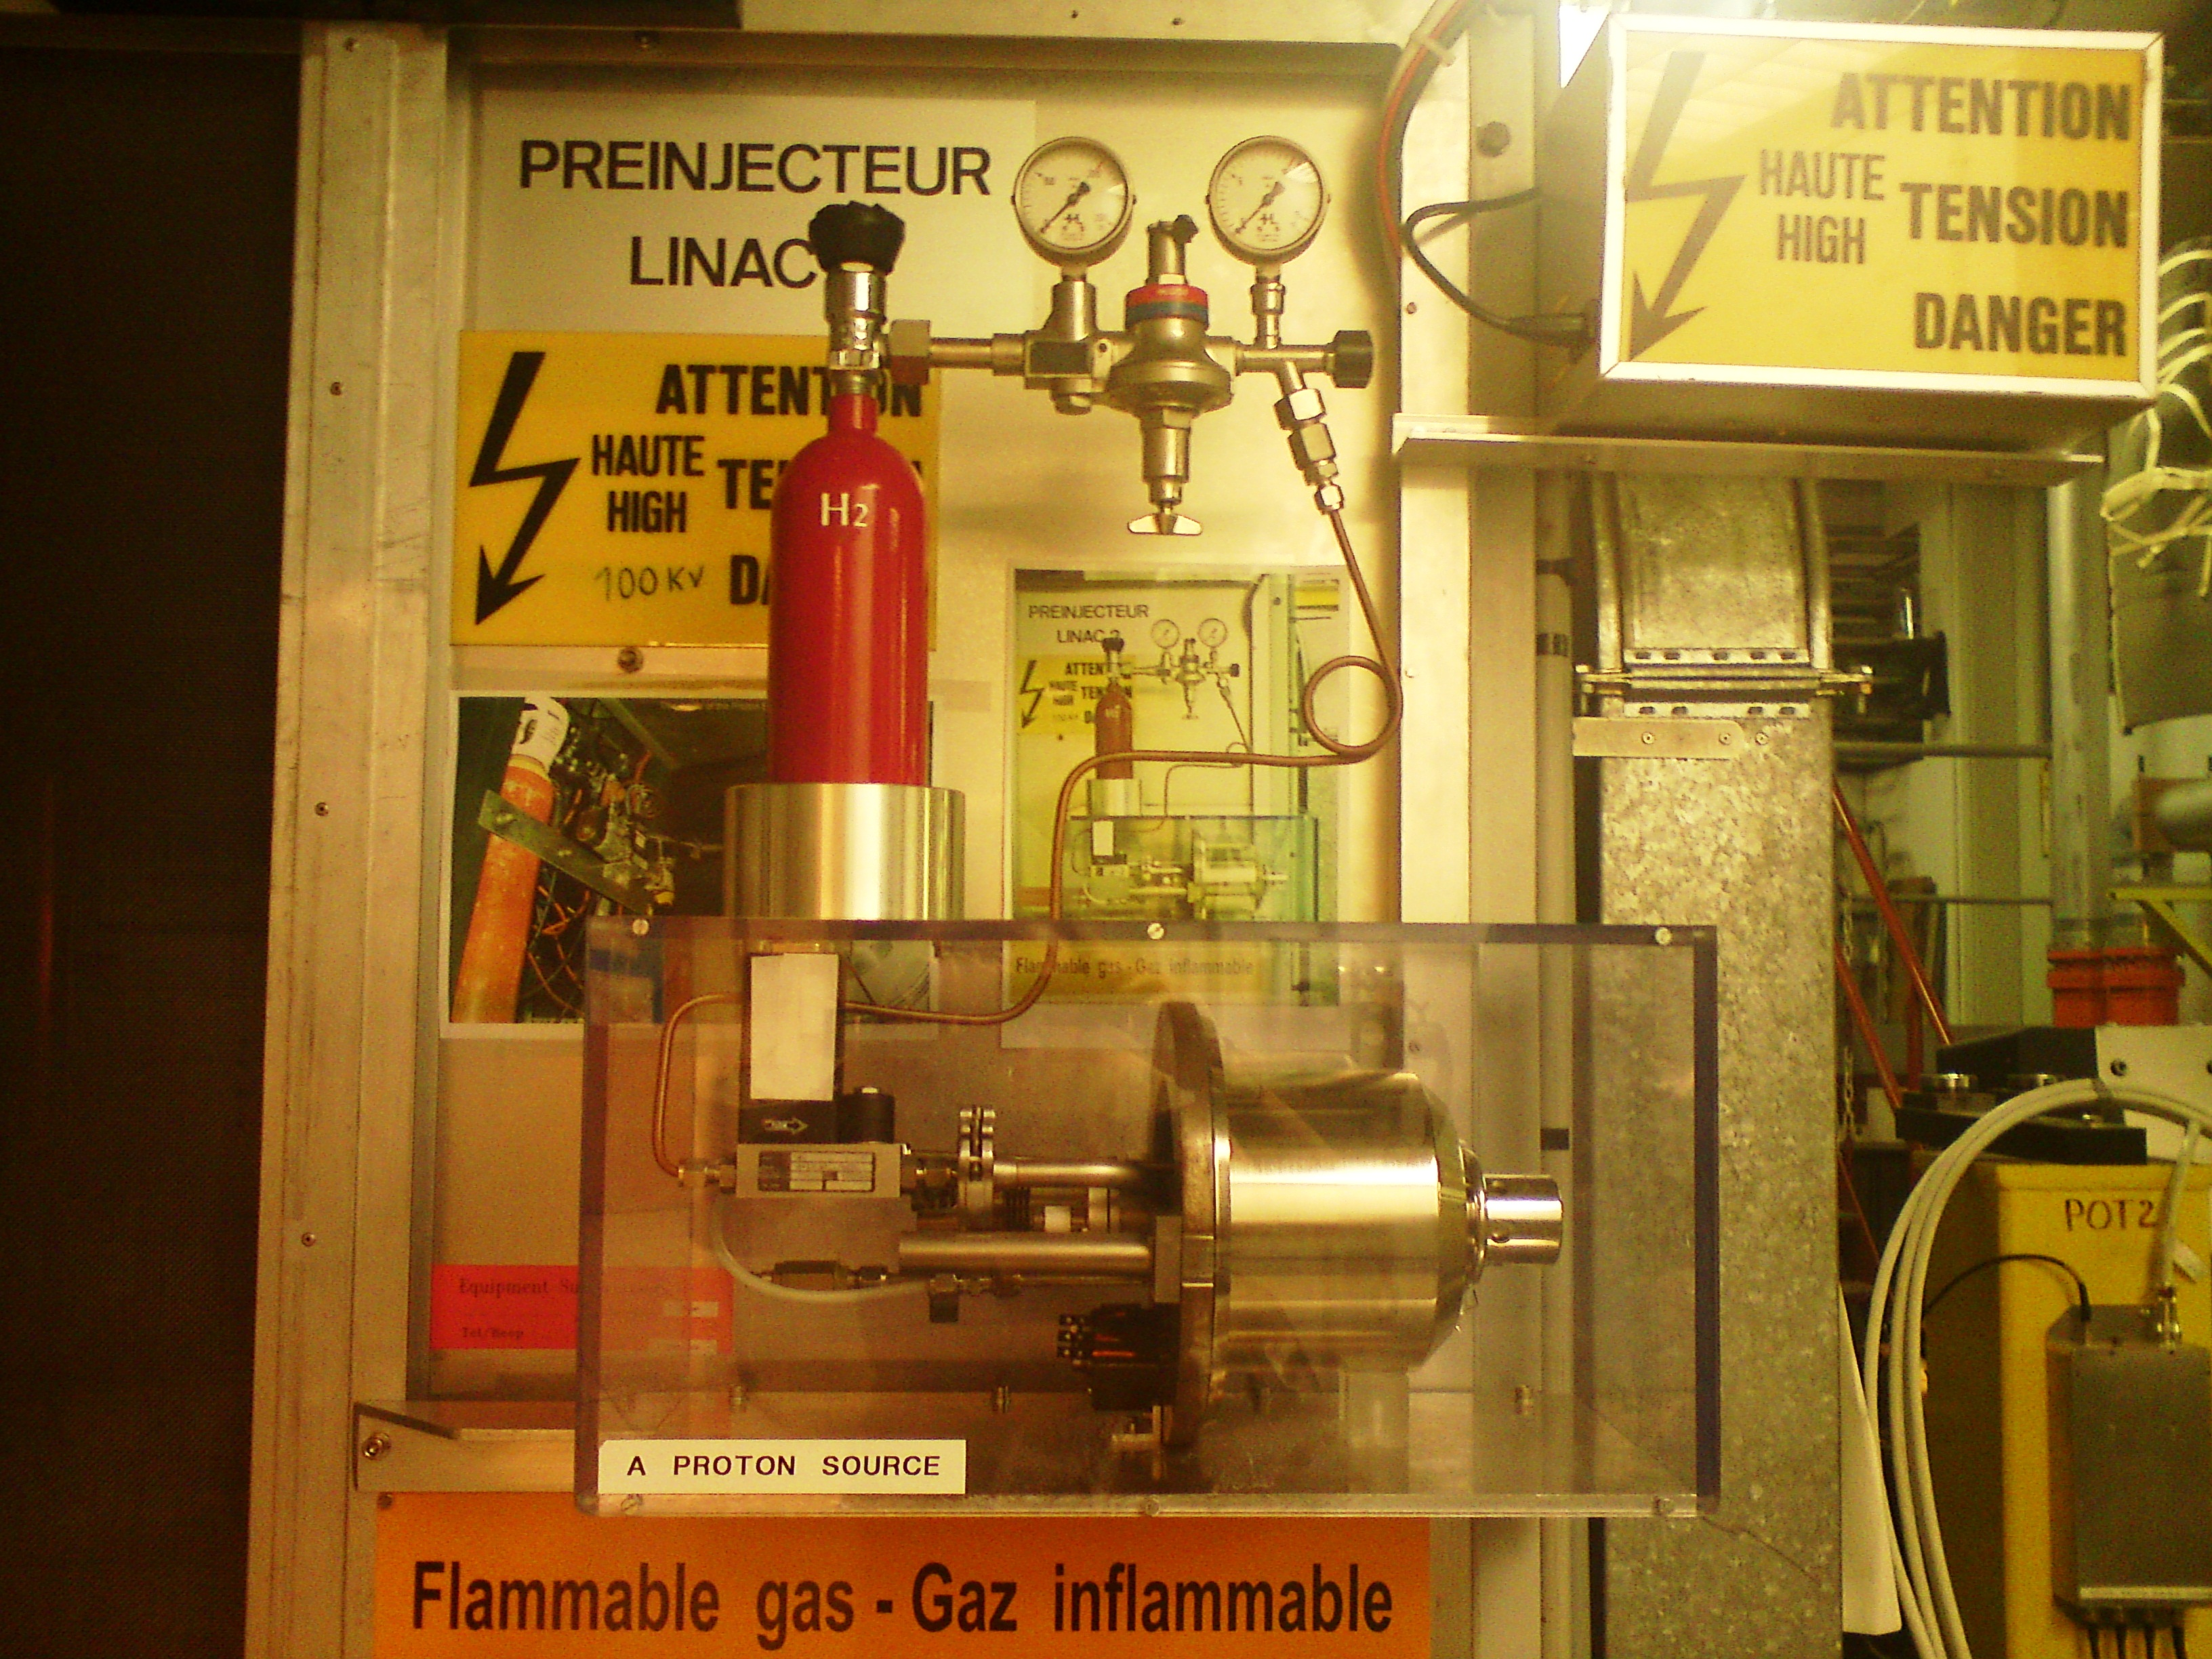
\includegraphics[width=\marginparwidth]{LHC/Bouteille.jpg}
	\label{bouteille}
    	\captionof{figure}{Source des protons du LHC.}
}	
\end{minipagewithmarginpars}

\marginpar
{
	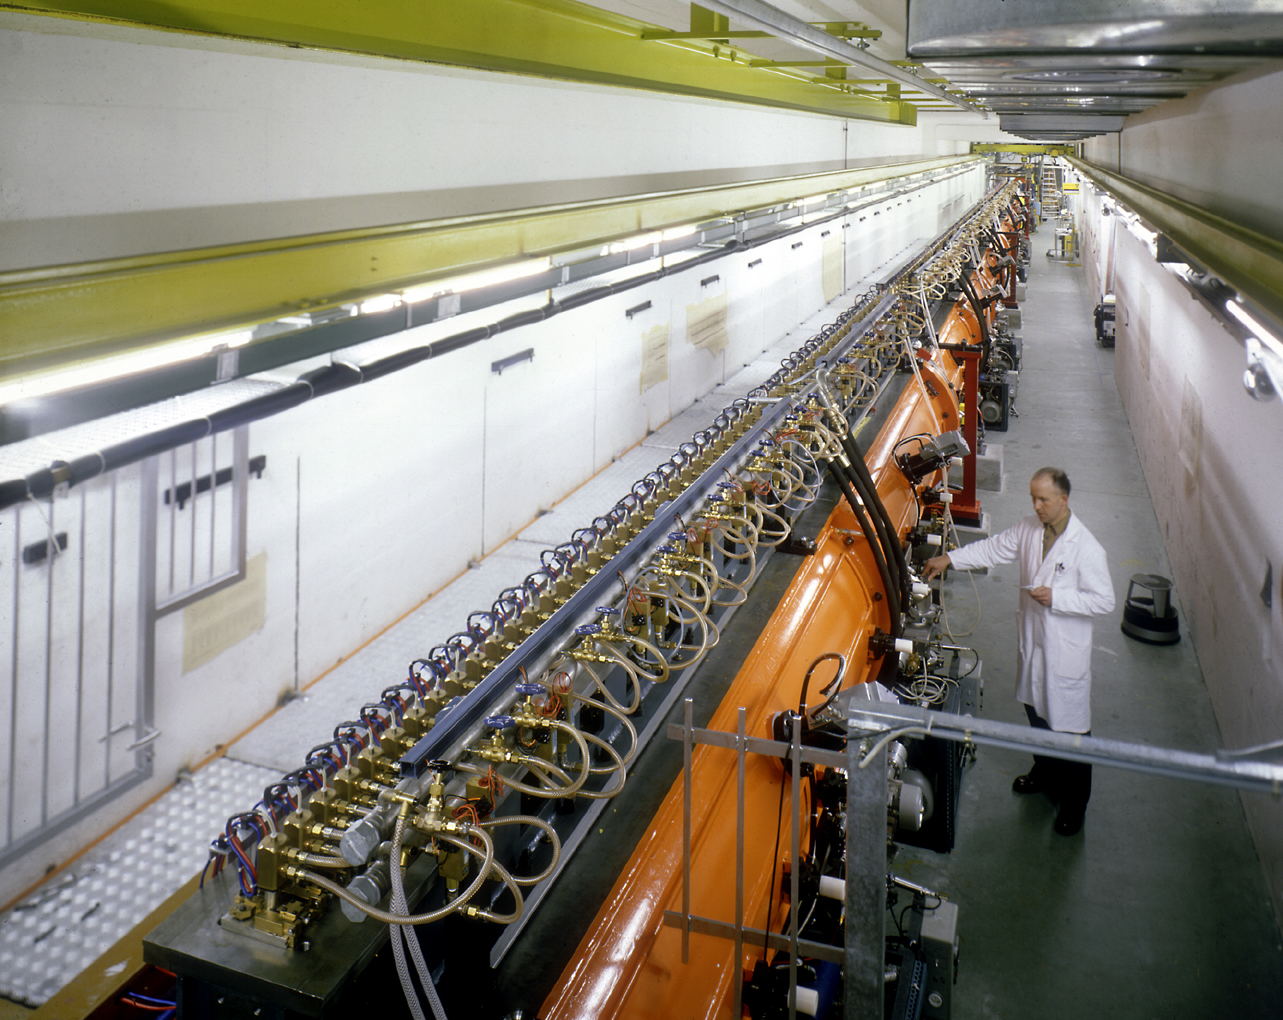
\includegraphics[width=\marginparwidth]{LHC/linac2.jpg}
    \captionof{figure}{Photo du LINAC 2.}
    	\label{linac2}
}

\marginpar
{
	
	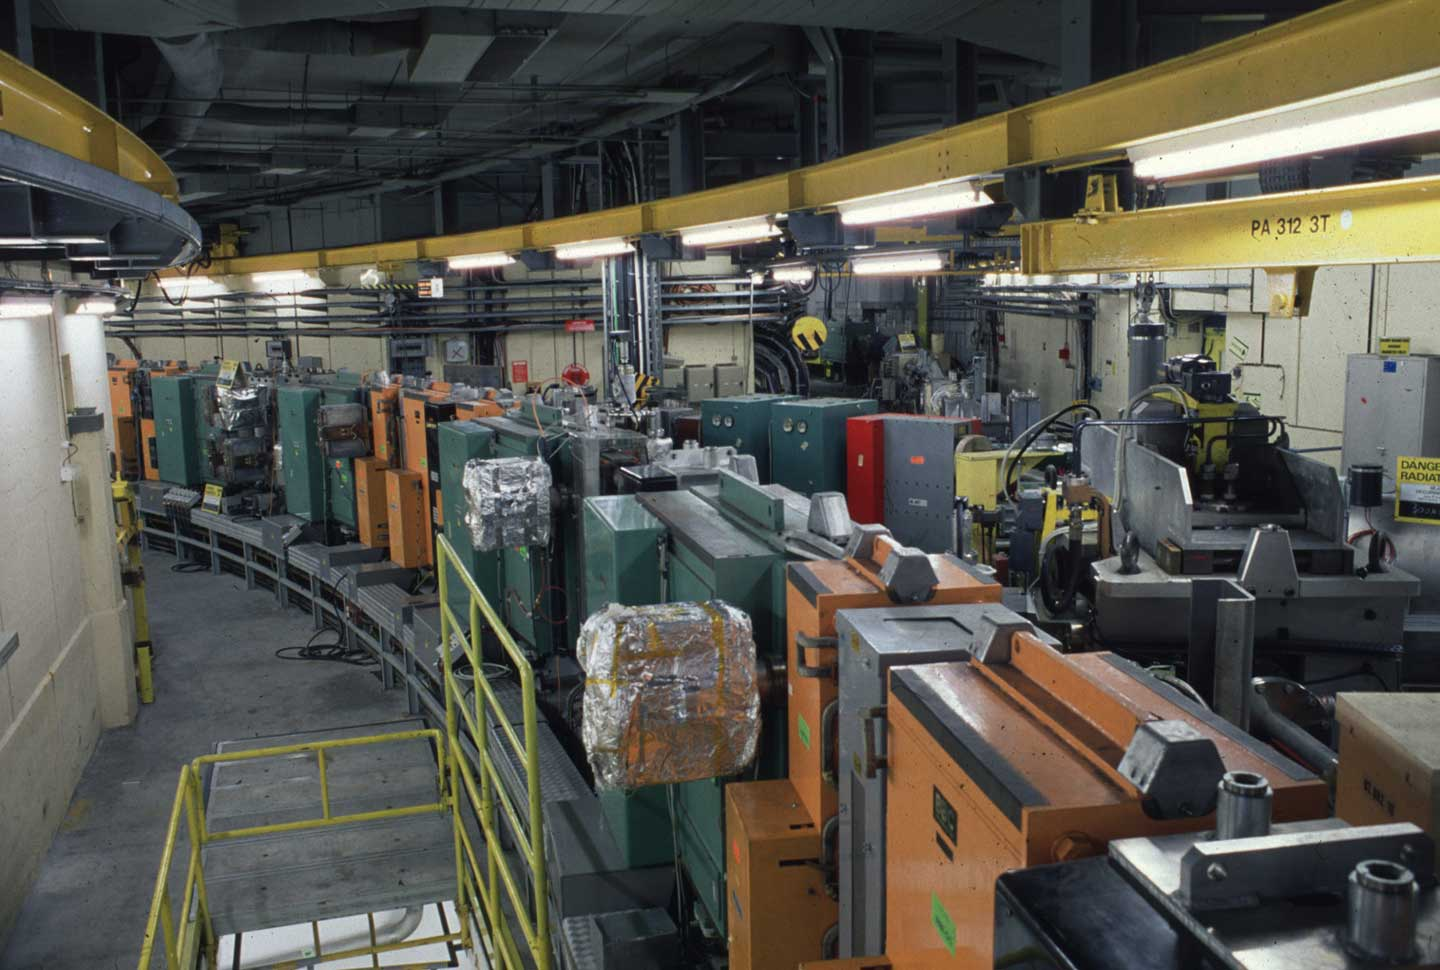
\includegraphics[width=\marginparwidth]{LHC/booster.jpg}
    \captionof{figure}{Photo du Booster du Synchrotron à protons.}
    	\label{booster}
}

\marginpar
{
	
	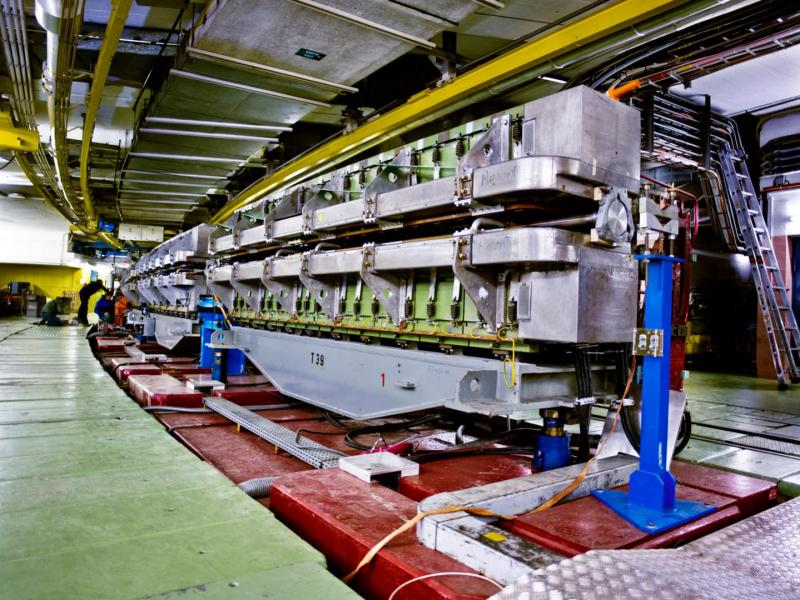
\includegraphics[width=\marginparwidth]{LHC/ps.jpg}
    \captionof{figure}{Photo du PS.}
    	\label{ps}
}

\marginpar
{
	
	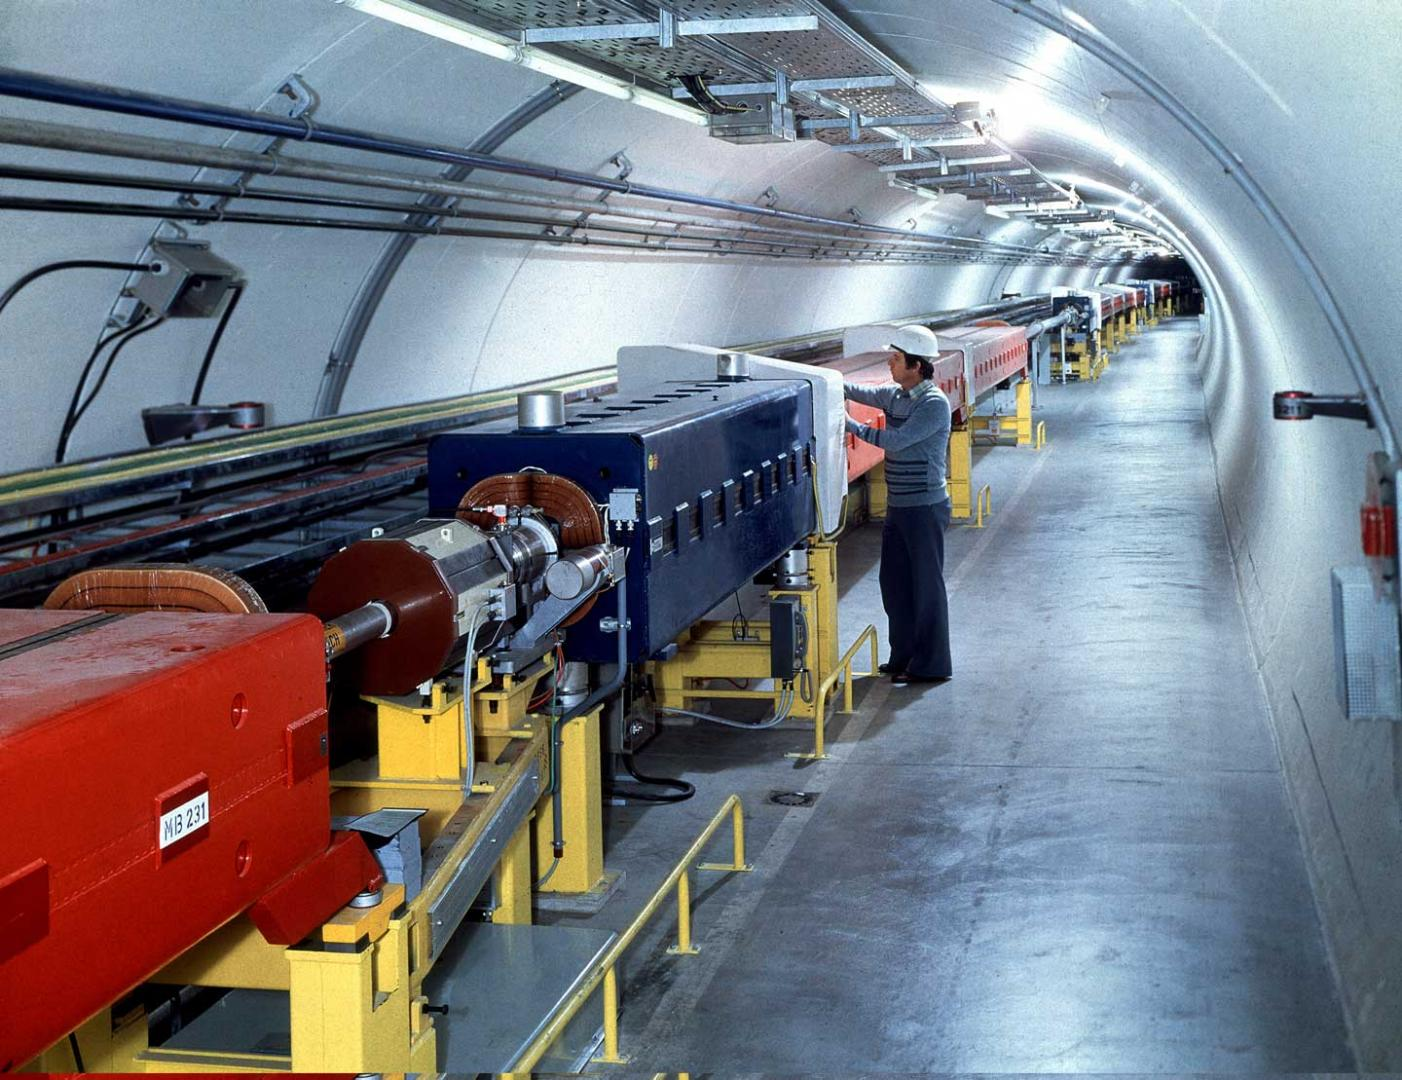
\includegraphics[width=\marginparwidth]{LHC/sps.jpg}
    \captionof{figure}{Photo du SPS.}
    	\label{sps}
}
Pour les collisions proton-proton, la source de protons est une bouteille de dihydrogène gazeux (fig. \ref{bouteille}). Les atomes d’hydrogène sont injectés dans le Duoplasmatron Proton IOn Source où il sont chauffés et sont soumis à un champ électrique, qui arrache leurs électrons et les ionise en $H^{+}$ (proton). Les protons extraits sont ensuite envoyés dans l'accélérateur linaire (LINAC 2 (fig. \ref{linac2})) où ils atteignent l'énergie de 50 MeV et sont $5\%$ plus massifs, leur vitesse est alors d'environ $0.3$c où c est la vitesse de la lumière dans le vide (c=$299 792 458$ m/s). Ils passent ensuite dans les 4 anneaux de 157m de circonférence du Booster du Synchrotron à protons (BOOSTER (fig. \ref{booster})) qui les amènent à une énergie de 1.4 GeV avant de les injecter dans l'accélérateur suivant, le Synchrotron à protons (PS (fig. \ref{ps})). Cet accélérateur circulaire de 628 mètres de circonférence, permet aux faisceaux d'atteindre une énergie de 25 GeV, leur vitesse est alors de 0.87c. Il sert aussi à préparer le faisceau en le découpant en série de paquets (bunchs) de particules nécessaires au LHC. Ces bunchs sont ensuite envoyés dans le supersynchrotron à protons (SPS (fig. \ref{sps})) d'une circonférence de 7 km, où l'énergie du faisceau atteint 450 GeV soit une vitesse de 0.99c. Les paquets sont regroupés pour former des trains de paquets avant d'être enfin envoyés dans le Grand Collisionneur de Protons (LHC). L'injection et le guidage de faisceaux d'une telle énergie par des aimants supraconducteurs rapides est une tâche délicate et pourrait détériorer l'accélérateur. Un faisceau de test de faible intensité "pilot beam" est donc injecté afin de mesurer et vérifier les paramètres. Le faisceau de haute énergie est ensuite séparé en deux et injecté dans deux conduits différents, l'un circulant dans un sens et l'autre dans le sens contraire. Ces faisceaux sont ensuite accélérés jusqu'à une énergie de 7 TeV et ne se croisent qu'aux points d'intéractions. À ce stade, les protons on une vitesse de 0.999999991c, soit 299 792 455,3 m/s. Il ne se déplace que 2.7m/s moins vite que la lumière. Afin d'accélérer les protons à une vitesse si proche de la lumière, d'importantes contraintes de pressions et de température sont nécessaires. Un vide poussé est nécessaire à l'intérieur du LHC afin de minimiser les interactions, la pression interne est de l'ordre de $10^{-13}$atm soit 10fois moins que la pression à la surface de la Lune. La présence d'aimants supraconducteurs nécessite un système de distribution cryogénique, qui assure la circulation d'hélium super-fluide est maintient le LHC à une température de $-271,3$\degre C ($1.9$K). Le LHC est donc plus froid que l'Univers (Le fond diffus cosmologique à en effet été évalué par le satellite Plank (cf.fig\ref{Plank}) (2009-2013) à $2,725$K.

\section{Le Large Hadron Collider}
Le LHC est le dernier accélérateur circulaire du complexe d'accélération.C'est actuellement le collisionner le plus puissant du monde (cf.fig\ref{livingston}) Il utilise le tunnel de 27 km de circonférence situé à une centaine de mètres sous terre. Il fût construit pour acceuillir le Grand collisionneur électron-positron (LEP\footnote{Large Electron Positron collider.}), qui fût en service de 1989 à 2000. Le LHC à été mis en service en 2008 et a été construit afin de produire de l'ordre de 600 millions de collisions proton-proton par seconde à une énergie au centre de masse de $\sqrt{s}=14$ TeV. Il est actuellement l'accélérateur de proton-proton le plus puissant du monde, et a permis de mettre en évidence l'existence du boson de Higgs, dernière pièce manquante du Modèle Standard.

Le LHC est un collissioneur de particules non fondamentales (hadrons) à l'inverse de son prédécesseur, le LEP qui utilisé des électrons et des positrons. Lors d'une collission entre hadrons, ceux sont ses constituant élementaires, les quarks et les gluons qui collissionnent entre eux. Ceux-ci possèdent seulement une portion de l'énergie du hadrons qui les contient. L'énergie du centre de masse de cette collision n'est donc pas connue avec précision. Le LHC est donc une machine de découverte de particules plutôt qu'une machine de mesures de précisions comme l'était le LEP, car il permet d'acceder à un large spectre en énergie. Généralement, les mesures de précision sont effectué grâce à des collisionneur utilisant des particules élémentaires ($e^{-}$,$e^{+}$); ils sont dans ce cas souvent linéaire afin d'éviter la perte d'énergie par rayonnement synchroton.

\begin{minipagewithmarginpars}[h]{0.95\textwidth}
	\centering
	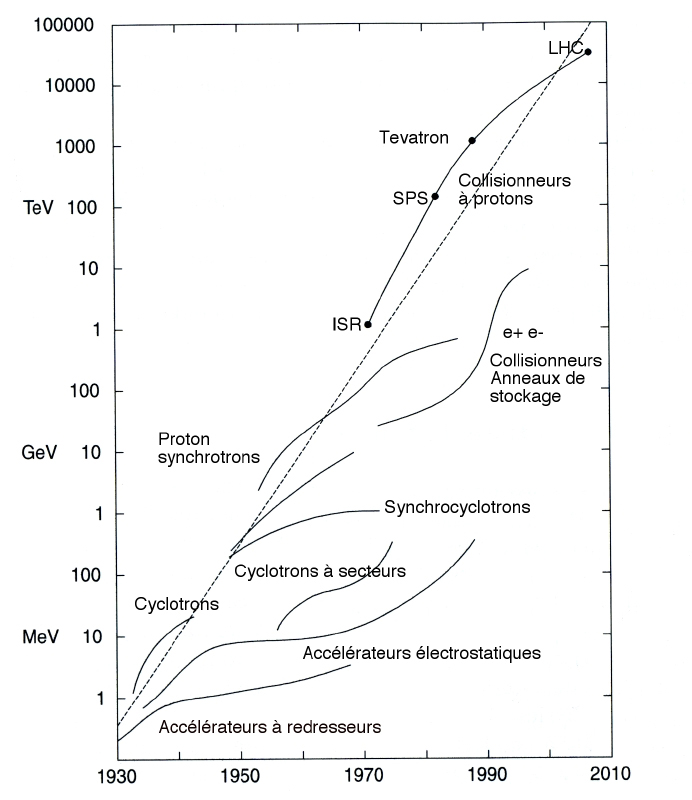
\includegraphics[width=0.8\textwidth]{LHC/Livingstone.jpg}
	\captionof{figure}{Diagramme de Livingston : Énergie des  faisceau de particules accélérées pour différentes machines en fonction du temps. Afin de pouvoir comparer les différents accélérateurs et technologies, l'énergie des collisionneurs, qui s'exprime dans le centre de masse, a été recalculée comme si l'énergie des particules observées était le résultat d'une collision avec un proton au repos (cible fixe).}
	\label{livingston}	
\end{minipagewithmarginpars}

La figure \ref{lhcschema} est une vue schématique du LHC. En vérité le LHC n'est pas parfaitement circulaire, mais est composé de $8$ octants composés d'une section droite de longueur $~5$ km et d'un secteur courbe d'une longueur de $~3$ km (fig. \ref{octants}). Afin de courber les faisceaux 1232 aimants dipolaires de 15 mètres de long sont utilisés et 392 aimants quadripolaires de 5 à 7 mètres servent à concentrer les faisceaux. Les sections droites sont utilisées afin de faire collisionner les deux faisceaux de protons venant en sens inverse l'un de l'autre. Il existe $8$ points potentiels d'interactions (P), mais seulement $4$ sont le siège de collisions et possèdent des détecteurs qui analysent les données issues de ces collisions : le point P1 pour ATLAS\footnote{A Toroidal LHC ApparatuS, détecteur généraliste.}, le point P2 pour ALICE\footnote{A Large Ion Collider Experiment, dédié à l'étude du plasma de quarks et gluons.}, le point P5 pour CMS\footnote{Compact Muon Solenoid, détecteur généraliste.} et le point P8 pour LHCb\footnote{Large Hadron Collider beauty experiment, dédié au quark b.}.

\marginpar
{
	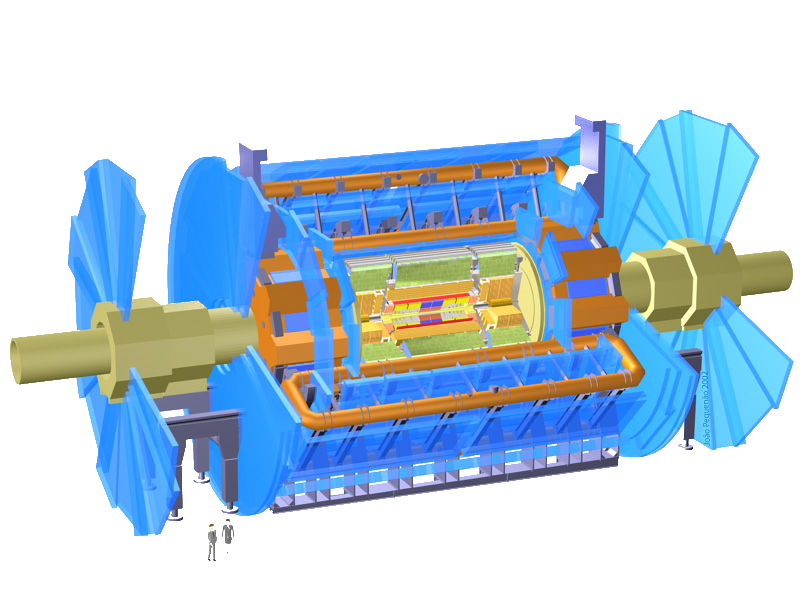
\includegraphics[width=\marginparwidth]{LHC/atlas.png}
    \captionof{figure}{ATLAS.}
    	\label{atlas}
}
\marginpar
{
	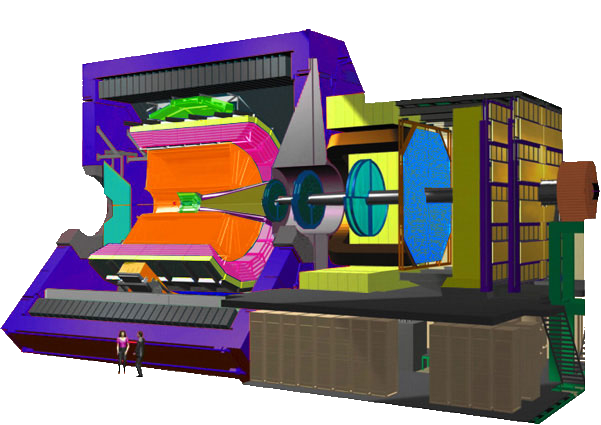
\includegraphics[width=\marginparwidth]{LHC/alice.png}
    \captionof{figure}{ALICE.}
    	\label{alice}
}
\marginpar
{
	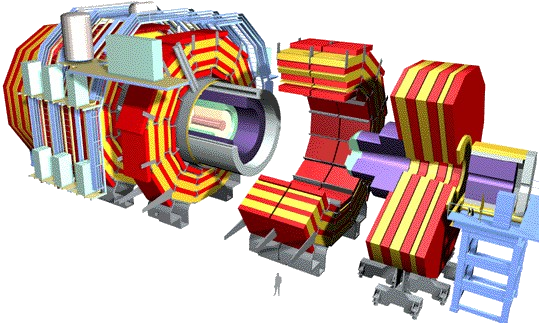
\includegraphics[width=\marginparwidth]{LHC/cms.png}
    \captionof{figure}{CMS.}
    	\label{cms}
}
\marginpar
{
	
	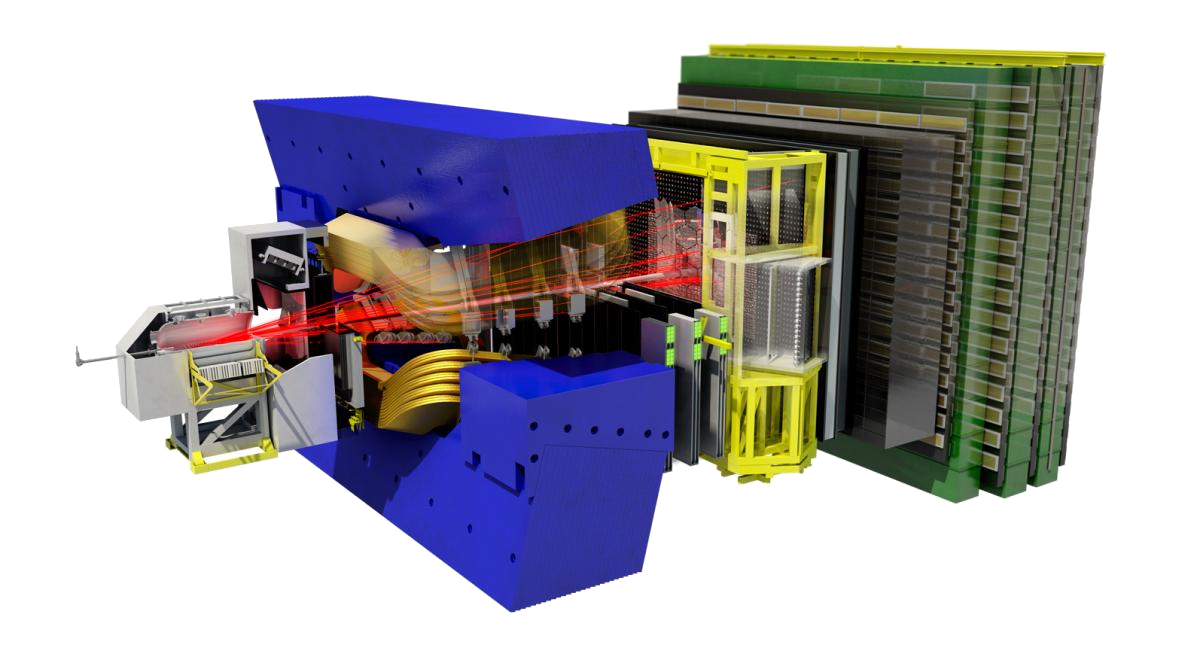
\includegraphics[width=\marginparwidth]{LHC/lhcb.png}
    \captionof{figure}{LHCb.}
    	\label{lhcb}
}

\begin{minipagewithmarginpars}[h]{\textwidth}
  	\centering
	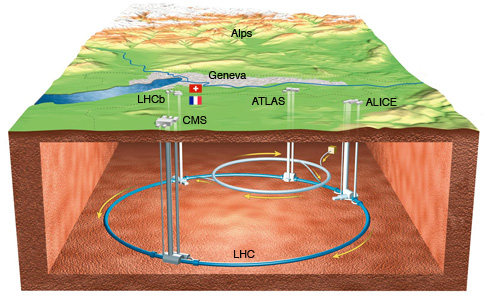
\includegraphics[scale=0.7]{LHC/CERNMap.jpg}
  	\captionof{figure}{Vue schématique du LHC.}
  	\label{lhcschema}	
\end{minipagewithmarginpars}

\begin{minipagewithmarginpars}[h]{0.95\textwidth}
  	\centering
	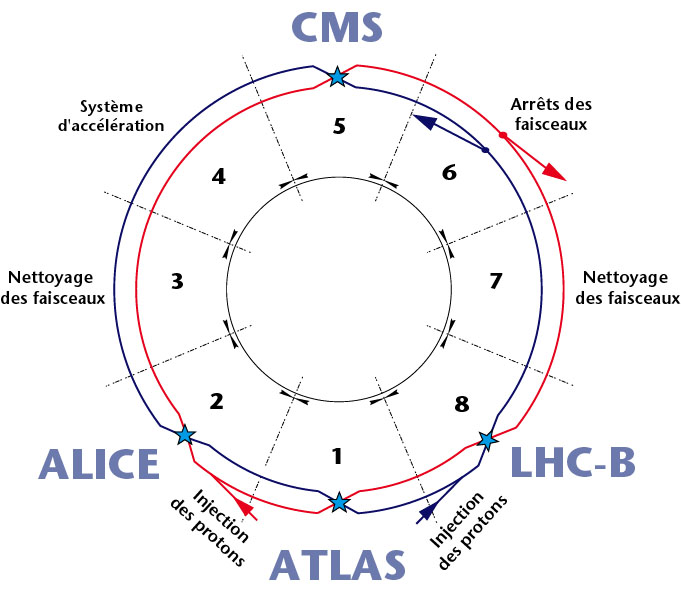
\includegraphics[width=0.75\textwidth]{LHC/lhc-schematic.jpg}
  	\captionof{figure}{Vue schématique des octants du LHC ainsi que des positions des principaux détecteurs le long du LHC. Les faisceaux (en bleu et rouge) circulent en sens inverse l'un de l'autre.}
  	\label{octants}	
\end{minipagewithmarginpars}

La réutilisation du tunnel du LEP et l'énergie des faisceau (7 TeV) à obligé l'utilisation d'aimant supraconducteur produsant des champs magnétique de 8.4T. De plus l'utilisation de deux faisceaux de protons voyant en sens inverse et l'espace limité dans le tunnel à amené à la création d'un nouveau type d'aimants où les deux tubes contenant les deux faisceaux sont insérés dans un même cryostat (cf.fig\ref{dipole}).

\begin{minipagewithmarginpars}[h]{0.95\textwidth}
\centering
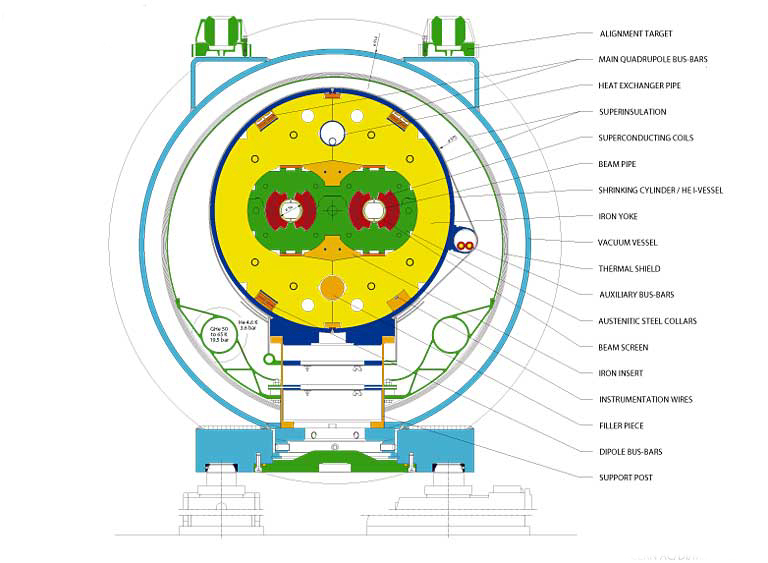
\includegraphics[width=0.85\textwidth]{LHC/dipole.jpg}
\captionof{figure}{Vue en transversale d'un dipole du LHC.}
\label{dipole}	
\end{minipagewithmarginpars}

\subsection{Luminosité des faisceaux}
Le nombre d'événement correspondant à un processus donnée que peut produire le LHC peut être exprimé par :
\begin{equation}
N=\int \mathcal{L}(t)\sigma \mathrm dt
\end{equation}
où $\sigma$ est la section efficace du processus considéré ( la probabilité q'un événement produise ce processus ), $t$ la durée de prise de donnée et $\mathcal{L}$ la luminosité instantanée délivré par la machine.

La luminosité est déterminée par les paramètres des faisceaux de protons :
\begin{equation}
\mathcal{L}=\frac{f_{rev}n_{p}N_{}}{4\pi \sigma_{x} \sigma_{y}} F(\phi)
\end{equation}
avec $N_{f}$ le nombre de protons par paquet, $n_{p}$ le nombre de paquets, $f_{rev}$ la fréquence de rotation d'un paquet, $\sigma_{x}$,($\sigma_{y}$) la moyenne quadratique horizontale (verticale) transverse de la taille du faisceau au point d'intéraction et $F(\phi)$ est le facteur de réduction géométrique définit en fonction de l'angle $\phi$ de Piwinski.
\begin{equation}
F(\phi)=\frac{1}{\sqrt{1+\phi^{2}}}
\end{equation}
En considérant des faisceau se croisant dans le plan verticale (cf.fig\ref{collision}), l'angle de Piwinski peut s'écrire :
\begin{equation}
\phi=\frac{\theta_{c}\sigma_{z}}{2\sigma_{y}}
\end{equation}
avec $\theta_{c}$ l'angle de croisement des faisceaux, $\sigma_{z}$ la moyenne quadratique de la longueur d'un paquet.


\begin{minipagewithmarginpars}[h]{0.95\textwidth}
\centering
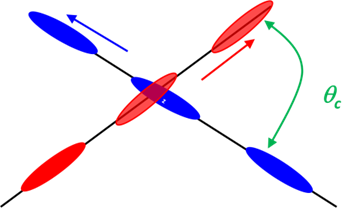
\includegraphics[width=0.35\textwidth]{LHC/collision.png}
\captionof{figure}{Schéma de colisions de paquets dans le plan transversale.}
\label{collision}	
\end{minipagewithmarginpars}

Il est possible d'exprimer $\sigma_{x}$ et $\sigma_{y}$ en fonction de l'émittance $\epsilon$ et de la fonction $\beta(s)$. L'émittance est l'espace dans l'espace des phase qui contientun certain pourcentage des particules du faisceau ( 95\% pour les collisionneur hadroniques). Elle est supposée constante durant toute la durée du temps de mesure \footnote{d'après le théorème de Liouville} :
\begin{equation}
\sigma_{x}=\sqrt{\epsilon\beta_{x}}
\end{equation}
avec s la postion le long de la trajectoire nominale du faisceau.

La valeur de la fonction $\beta$ au point d'interaction est noté $\beta^{*}$.En considérant de plus que $\sigma_{x}=\sigma_{x}=\sigma$ on peut réécrire $\mathcal{L}$ comme :
\begin{equation}
\mathcal{L}=\frac{f_{rev}\gamma\beta n_{p}N_{p}}{4\epsilon_{n}\beta^{*}\pi} F(\phi)
\end{equation}
où $\epsilon_{n}=\epsilon\gamma\beta$ est l'émittance normalisé, $\gamma$ le facteur de Lorentz $\beta=v/c$.

D'après cette formule on peut remarqué qu'il peut être interéssant de réduire au maximun $\epsilon_{n}$ c'est à dire d'avoir des paquet dont les particules ont la même quantité de mouvement et son proche l'une de l'autre. Il est aussi possible de réduire le facteur de réduction géométrique en utilisant une configuration de faisceau dite en "crabe" (cf.fig\ref{crabe})

\begin{minipagewithmarginpars}[h]{0.95\textwidth}
\centering
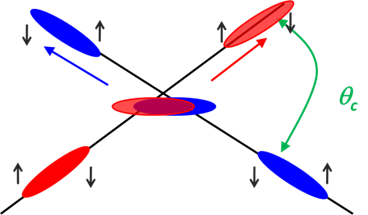
\includegraphics[width=0.35\textwidth]{LHC/crab.png}
\captionof{figure}{Schéma de colisions "en crab" de paquets dans le plan transversale.}
\label{crabe}	
\end{minipagewithmarginpars}

La luminosité du faisceau ne reste pas constante tout le long d'un cycle de prise de donnée. La cause principale sont les collisions dans les détecteurs.Le temps de décroissance caractéristique de l'intensité du faisceau par les collisions est :
\begin{equation}
\tau{collisions}=\frac{N_{0}}{L_{0}\sigma_{tot}n}
\end{equation}
avec $N_{0}$ le nombre de protons à l'injection, $L_{0}$ la luminosité initiale,$\sigma_{tot}$ la section efficace totale et $n$ le nombre de point d'interactions des faisceaux.

Les deux autres causes principales de la réduction de la luminosité des faisceaux sont d'une part la perte par interaction entres les particules du faisceaux et le gaz piégé dans les tubes (avec un temps caractéristique $\tau_{gaz}$) ainsi que par diverses perturbations et imperfections ( champ magnétique par exemple ) qui peuvent dévier les particules de la trajectoire nominale du faisceau ($\tau_{imper}$) . 
La décroissance de la luminosité instantanée peut être donné par la formule:
\begin{equation}
\frac{\mathrm \mathcal{L}}{\mathrm t} = L_{0} e^{-\frac{t}{\tau}}
\end{equation}
avec
\begin{equation}
\frac{1}{\tau} = \frac{1}{\tau_{collisions}}+\frac{1}{\tau_{gaz}}+\frac{1}{\tau_{imper}}
\end{equation}

Lorsque l'intensité du faisceau devient trop faible pour une prise de données efficace, les faisceaux sont déviés de leurs trajectoires circulaires et envoyé dans les "dump blocks" (cf.fig\ref{dump})
\marginpar
{
	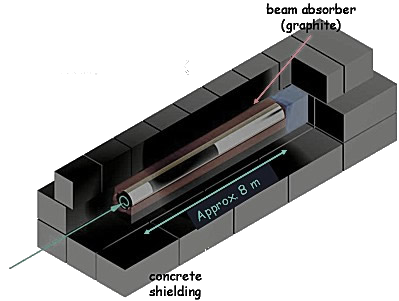
\includegraphics[width=\marginparwidth]{LHC/dump.png}
    \captionof{figure}{Schéma d'un "dump block".}
    	\label{dump}
}

La luminosité intégré pour les collisions protons-protons délivré par le LHC en 2016 ainsi que celle enregistré par  le détecteur CMS est donné par le graphique suivant :
\begin{minipagewithmarginpars}[h]{0.95\textwidth}
\centering
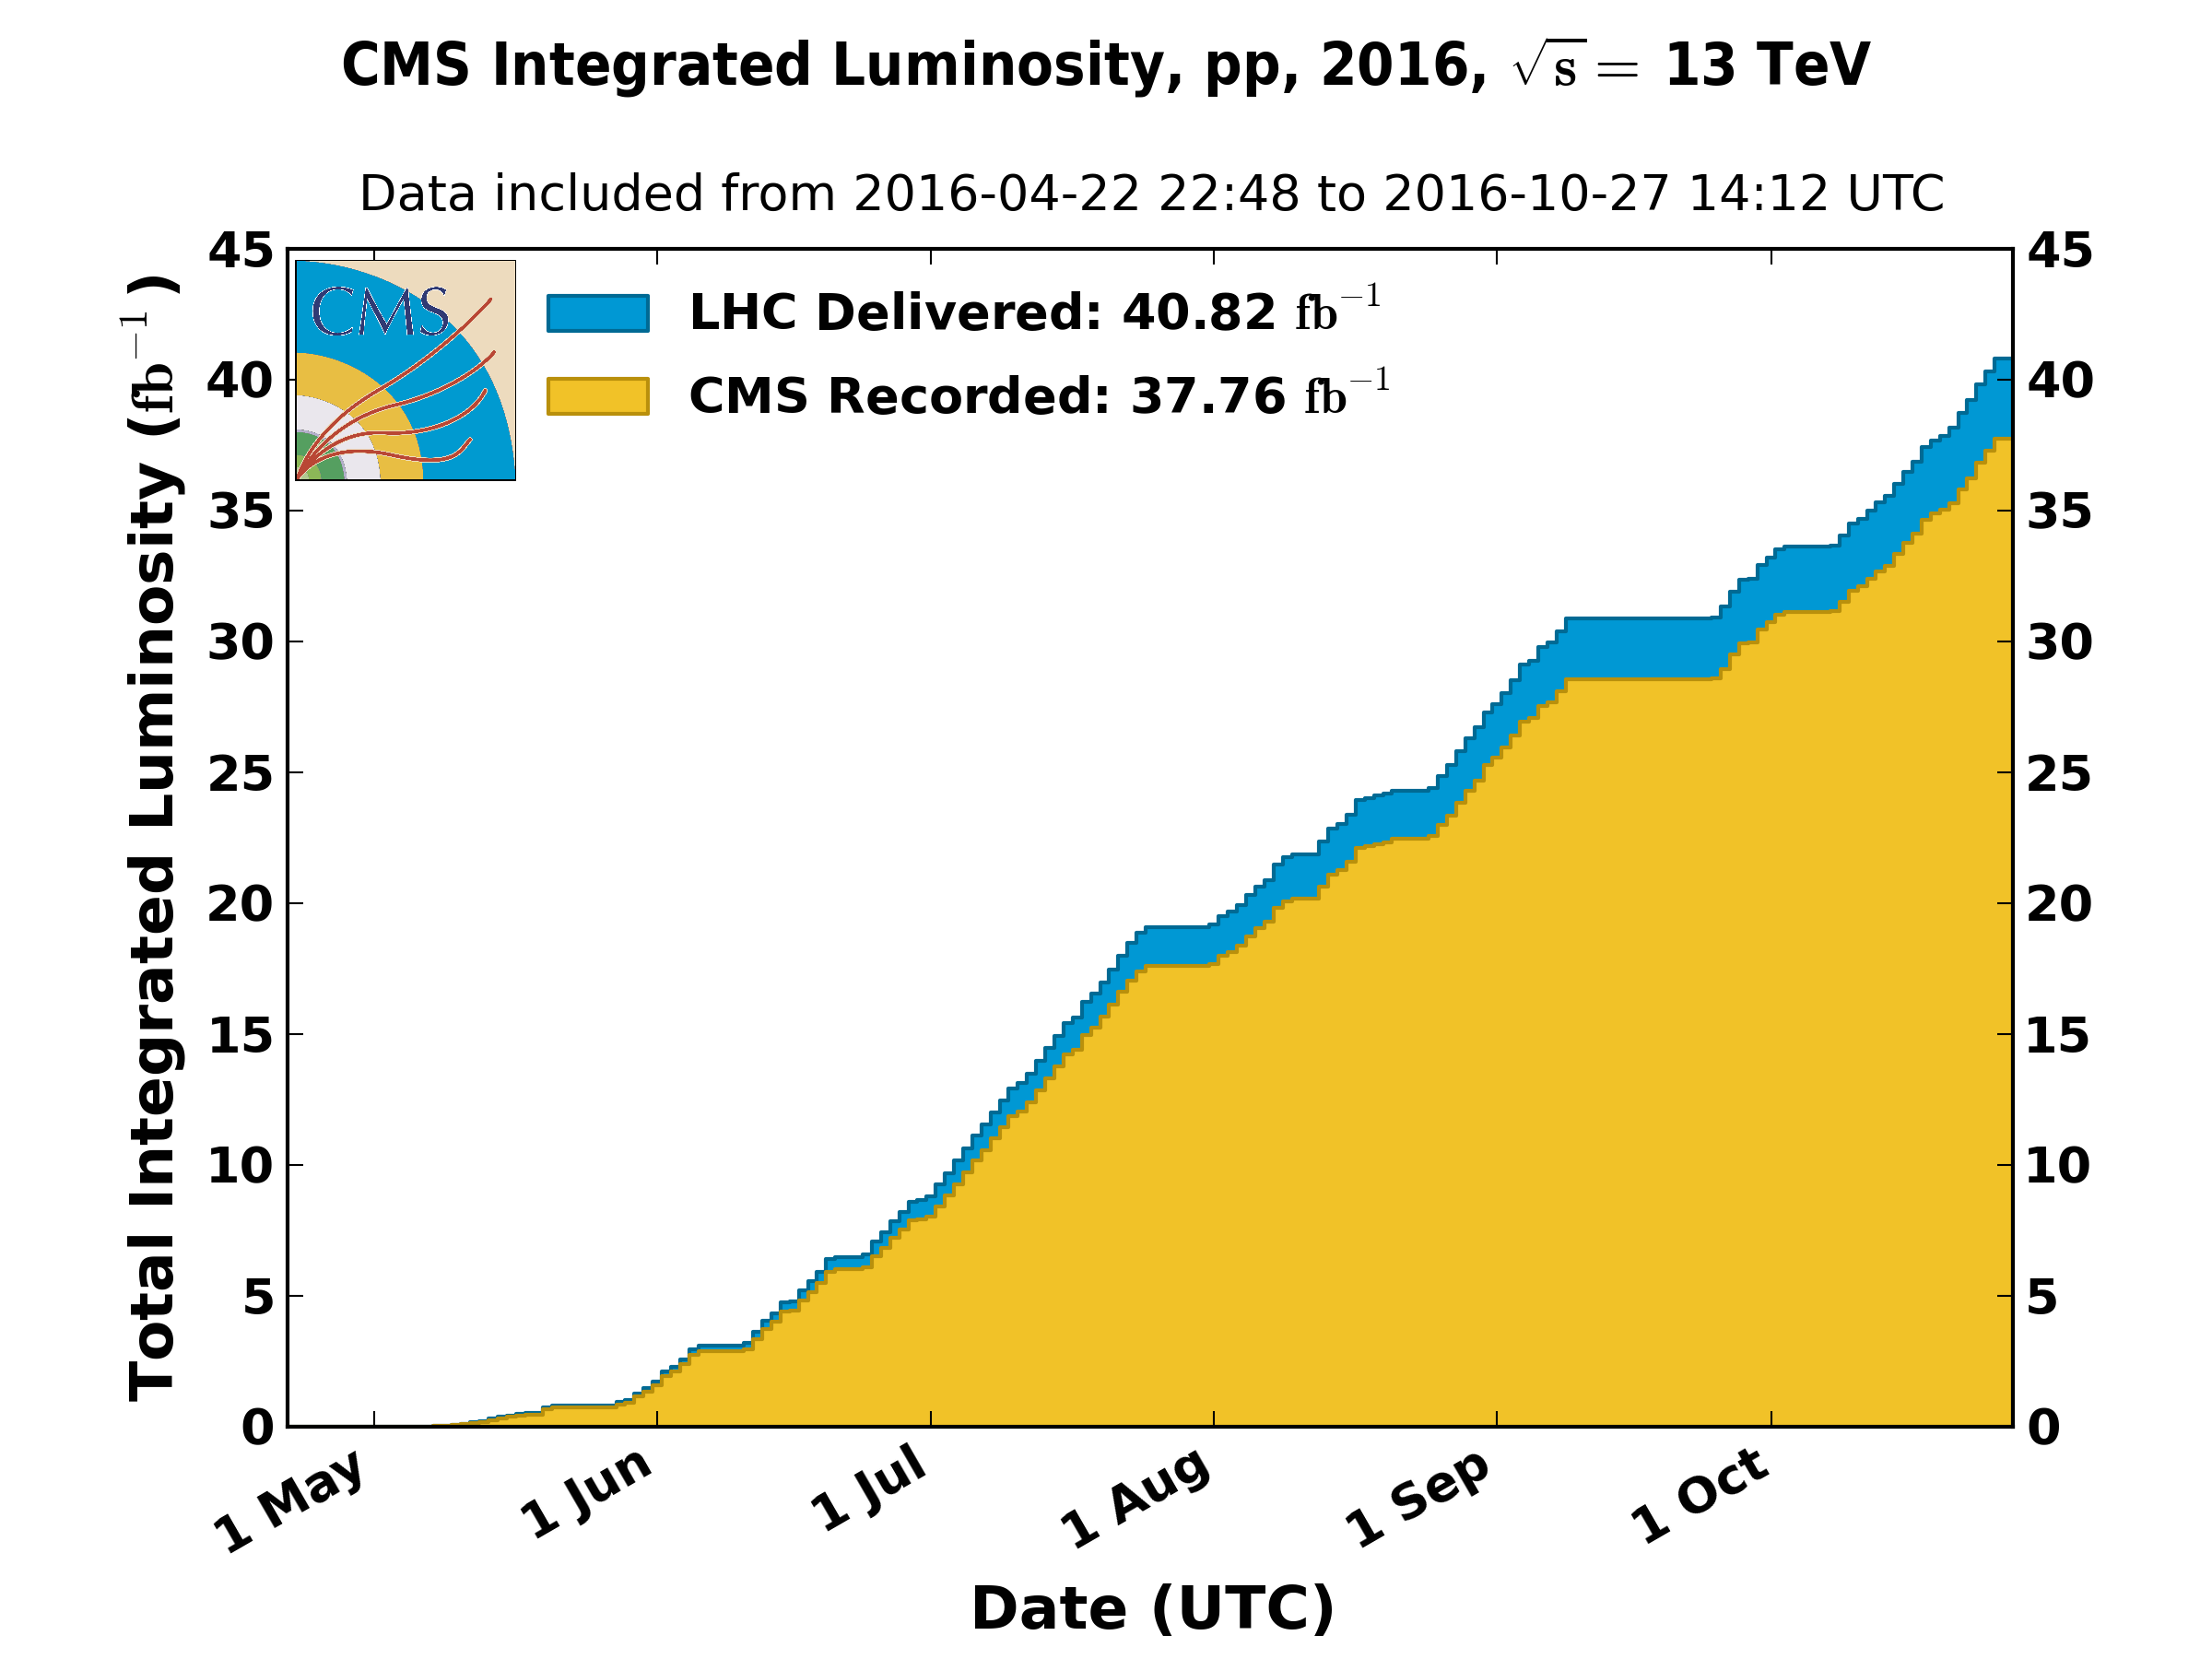
\includegraphics[width=0.7\textwidth]{LHC/luminosity.png}
    \captionof{figure}{Luminosité intégrée en fonction du jour de l'année 2016 délivrée (bleu) et enregistrée par CMS (orange) pendant les faisceaux stables et pour les collisions pp à 13 TeV d'énergie dans le centre de masse en 2016.}
\end{minipagewithmarginpars}

\subsection{Collisions protons-protons}
Le proton n'est pas une particule élémentaire. Il est composé de 3 quarks de valence (uud) et de quarks, antiquarks et gluons regroupés sous le termes de partons (cf.fig\ref{proton})

\begin{minipagewithmarginpars}[h]{0.95\textwidth}
\centering
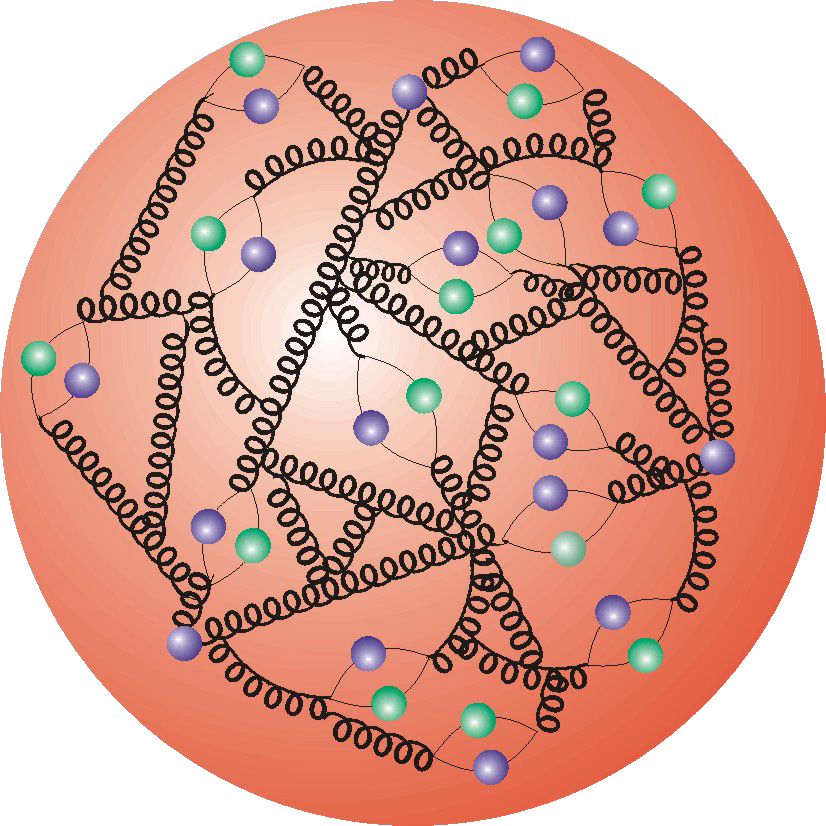
\includegraphics[width=0.3\textwidth]{SM/quarks3.png}
\captionof{figure}{Schéma d'un protons : les quarks (vert) et anti-quarks (bleu) sont en interactions par l'intermédiaire de gluons (noire).}
\label{proton}	
\end{minipagewithmarginpars}

Les collisions proton-proton peuvent être rassemblés en trois groupes :
\begin{itemize}[label=$\bullet$]
	\item \textbf{Les collisions élastiques : } Les collisions élastique préservent l'énergie cinétique totale des protons. Ces collisions ne sont pas intéressante pour la physique est ne font que pollués. Elle correspondes à des collisions de basse quantité de mouvement.
	\item\textbf{Les collisions diffractives : } Elles se produisent lorsque la quantité de mouvement des deux protons et plus importante. Elle se caractérise par la fragmentation d'un proton pour la diffraction simple ou des deux protons pour la diffraction double.
	\item \textbf{Les collisions inélastiques : } Ces collisions se produisent lorsque l'un des parton d'un proton interagit avec un parton de l'autre proton. Ce sont ces interactions à haute quantité de mouvement qui sont les plus intéressantes pour la recherche de nouvelle particules.
\end{itemize}

\subsubsection{Collisions inélastiques}
Les collisions inélastique se produisent entre deux partons qui possèdent une fraction de la quantité de mouvement $x_{1}$ et $x_{2}$ du proton $1$ et $2$. Ces fractions sont décrites par des fonctions de distribution de partons $f(x,Q^{2})$. Il s'agit des densités de probabilités de trouver une particule avec une fraction $x$ de la quantité de mouvement longitudinale du hadron dont l'impulsion est $Q^{2}$. Il existe une fonction de distribution de parton par saveur de quark et une pour les gluons (cf.fig\ref{pdf}). La figure \ref{pdf} représente ces fonctions.

\begin{minipagewithmarginpars}[h]{0.95\textwidth}
	\centering
	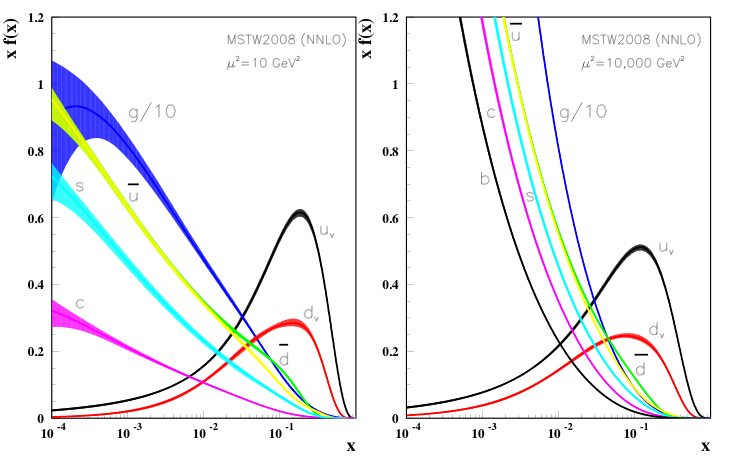
\includegraphics[width=0.9\textwidth]{LHC/pdf.png}
	\captionof{figure}{$x$ fois la  distribution de parton non-polarisé $f(x)$ ou $f=u_{v},d_{v},\bar{u},\bar{d},s,c,b,g)$ et leurs incertitudes en utilisant la parametrisation NNLO MSTW2008 à l'échelle $10$GeV$^{2}$ (gauche) $10000$GeV$^{2}$ (droite).}
	\label{pdf}	
\end{minipagewithmarginpars}
 
Ces fonctions ne peuvent être déduites que des données expérimentales car l'échelle d'énergie de QCD à laquelle sont soumis les partons au sein du proton ne permet pas d'effectuer un calcul perturbatif. On peut remarquer que la contribution des gluons est la plus importante et que les quarks de valence ont une contribution plus importantes que ceux de la mer de partons.

En utilisant ces fonctions et le théorème de factoriation de QCD, il est possible de calculer la section efficace d'un événement $A+B\rightarrow X$ par la formule :
\begin{equation}
\sigma_{A+B\rightarrow X}=\sum_{i=q,g}\int_{0}^{1} \mathrm{d}x_{a}\mathrm{d}x_{b}f_{a/A}(x_{a},\mu_{F}^{2})f_{b/B}(x_{b},\mu_{F}^{2})\sigma{_{a+b\rightarrow X}}
\end{equation}
L'échelle de factorisation $\mu^{2}$ est la limite entre la partie non perturbative $f_{b/B}(x_{b},\mu^{2})$ et la partie calculable par la théorie perturbative $\sigma{_{a+a\rightarrow X}}$.

Il est ainsi possible de calculer $\sigma{_{a+b\rightarrow X}}$ par la méthode perturbative et de la développer en terme de puissance de la constante de couplage $\alpha_{s}\left(\mu_{R}^{2}\right)$ qui dépend de l'échelle de renormalisation:
\begin{equation}
\sigma_{a+a\rightarrow X}=\left[\sigma_{0}+\alpha_{S}\left(\mu_{R}^{2}\right)\sigma_{1}+\cdots\right]_{a+b\rightarrow X}
\label{eq2}
\end{equation}
La figure fig.\ref{crosssection} montre quelques sections efficaces du Modèle Standard pour des collisions protons-protons protons-anti-protons calculés au "next-to-leading order" ($\sigma_{1}$ dans la formule \ref{eq2}).

\begin{minipagewithmarginpars}[h]{0.95\textwidth}
	\centering
	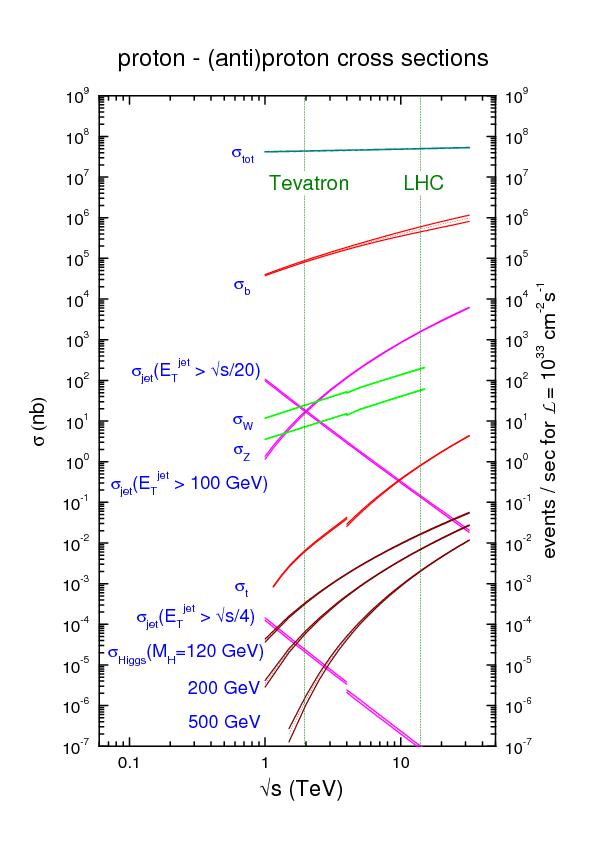
\includegraphics[width=0.6\textwidth]{LHC/crosssections2008.png}
	\captionof{figure}{Sections efficaces du Modèle Standard pour les collisionneurs LHC et Tevatron en fonction de l'énergie dans le centre de masse $\sqrt{s}$. Les lignes pointillées indiquent les énergies dans le centre de masse à laquelles le Tevatron (1.96TeV) et le LHC (7,10 et 14 TeV) vont foctionner. Les sections efficaces sont exprimées en nanobarn (gauche) et en Hz pour une luminositée instantannée de $\mathrm{L}=10^{33}$cm$^{-2}$s$^{-1}$, luminosité typique des premières années de fonctionnement du LHC.}
	\label{crosssection}	
\end{minipagewithmarginpars}

\subsection{Collisions proton-proton inélastiques}
Les collisions inélastiques sont le siège de plusieurs processus (fig\ref{collision2}). Parmis les plus important citons :
\begin{itemize}[label=$\bullet$]
	\item \textbf{La collision profondément inélastiques :} Deux partons très énergétique des deux protons rentre ne collision.
	\item \textbf{Les collisions sous-jacentes :} Plusieurs collisions entre les partons restant des protons peuvent avoir lieux.
	\item \textbf{Les radiations de l'état initial :} Avant l'interactions des deux partons responsable de la collsion principale, ces deux partons peuvent rayonnés des quarks et des gluons.
	\item \textbf{Les radiations finales :} Les particules crééent après la collsion principale peuvent elles-mêmes rayonner des quarks et des gluons.
	\item \textbf{L'hadronisation :} dû à la propriété du confinement, les quarks et gluons vont s'hadroniser afin de former des hadrons de couleur blanches qui formrnt des jets.
	\item \textbf{Les désintégrations :} Nombre des hadrons et mésons creés pendant le processus d'hadronisation ne sont pas stables et vont se désintégrer, parfois en cascade en particules stables.
\end{itemize}

\begin{minipagewithmarginpars}[h]{0.95\textwidth}
	\centering
	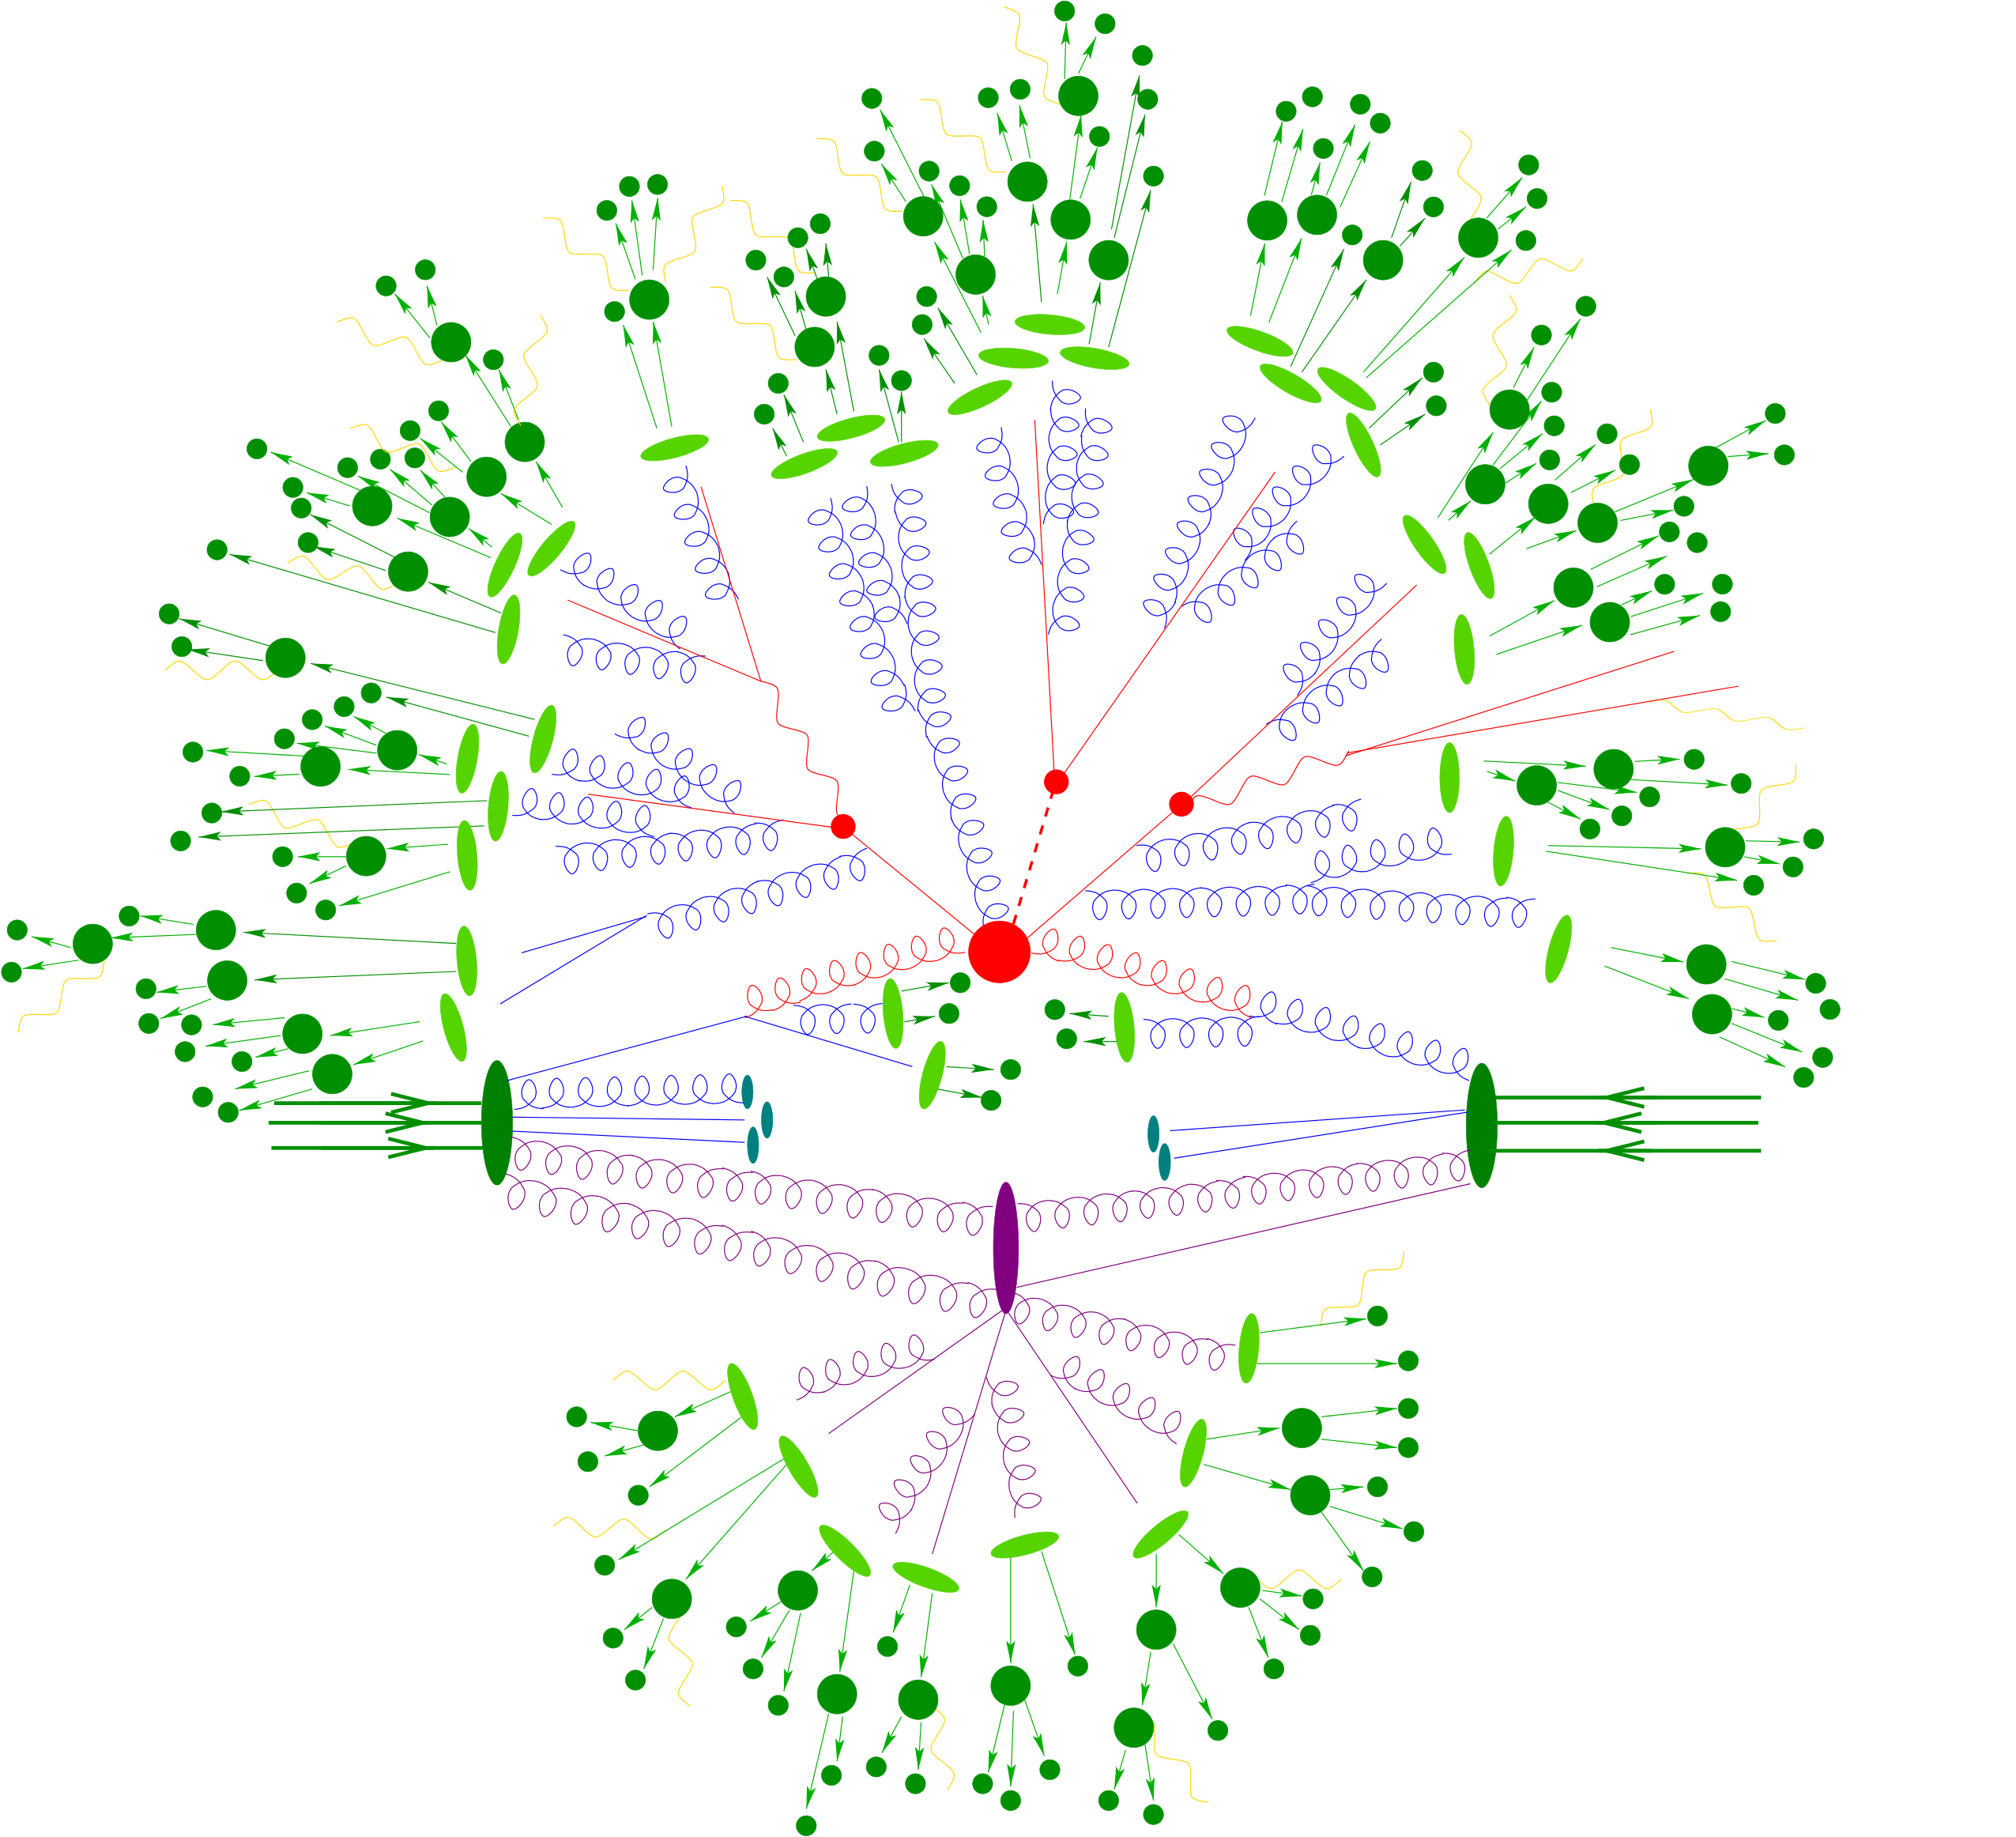
\includegraphics[width=0.7\textwidth]{LHC/event.jpg}
	\captionof{figure}{Schéma d'une collision proton-proton inélastique. Deux partons venant de deux protons différents interagissent inélastiquement (rouge), d'autres partons de ces deux protons produissent des collisions secondaires (magenta). Les partons ainsi créés s'hadronise (rouge) en creant des jets de particules (vert clair). Ces particules instables se désintégre en cascade en particules stables (vert foncé)}
	\label{collision2}	
\end{minipagewithmarginpars}

\subsection{L'empilement en temps et hors-temps}
Plusieurs collisions proton-proton peuvent avoir lieux lors d'un même croisement de faisceaux. Ces collisions appartiennent donc au même événement et forme un empilement en temp "on-time pile-up". De plus certaines désintégrations et phénoménes peuvent durée plus longtemps que le temps entre deux croisement de faisceaux. Ces événement sont appelés empilement hors-temps ou "off-time pile-up". Le phénomène d'empilement dépend de la luminosité et de l'énergie des faisceaux. La figure \ref{pile-up} montre la distribution du nombre d'événement par croisement de faisceaux dans CMS en 2012.

\begin{minipagewithmarginpars}[h]{0.95\textwidth}
	\centering
	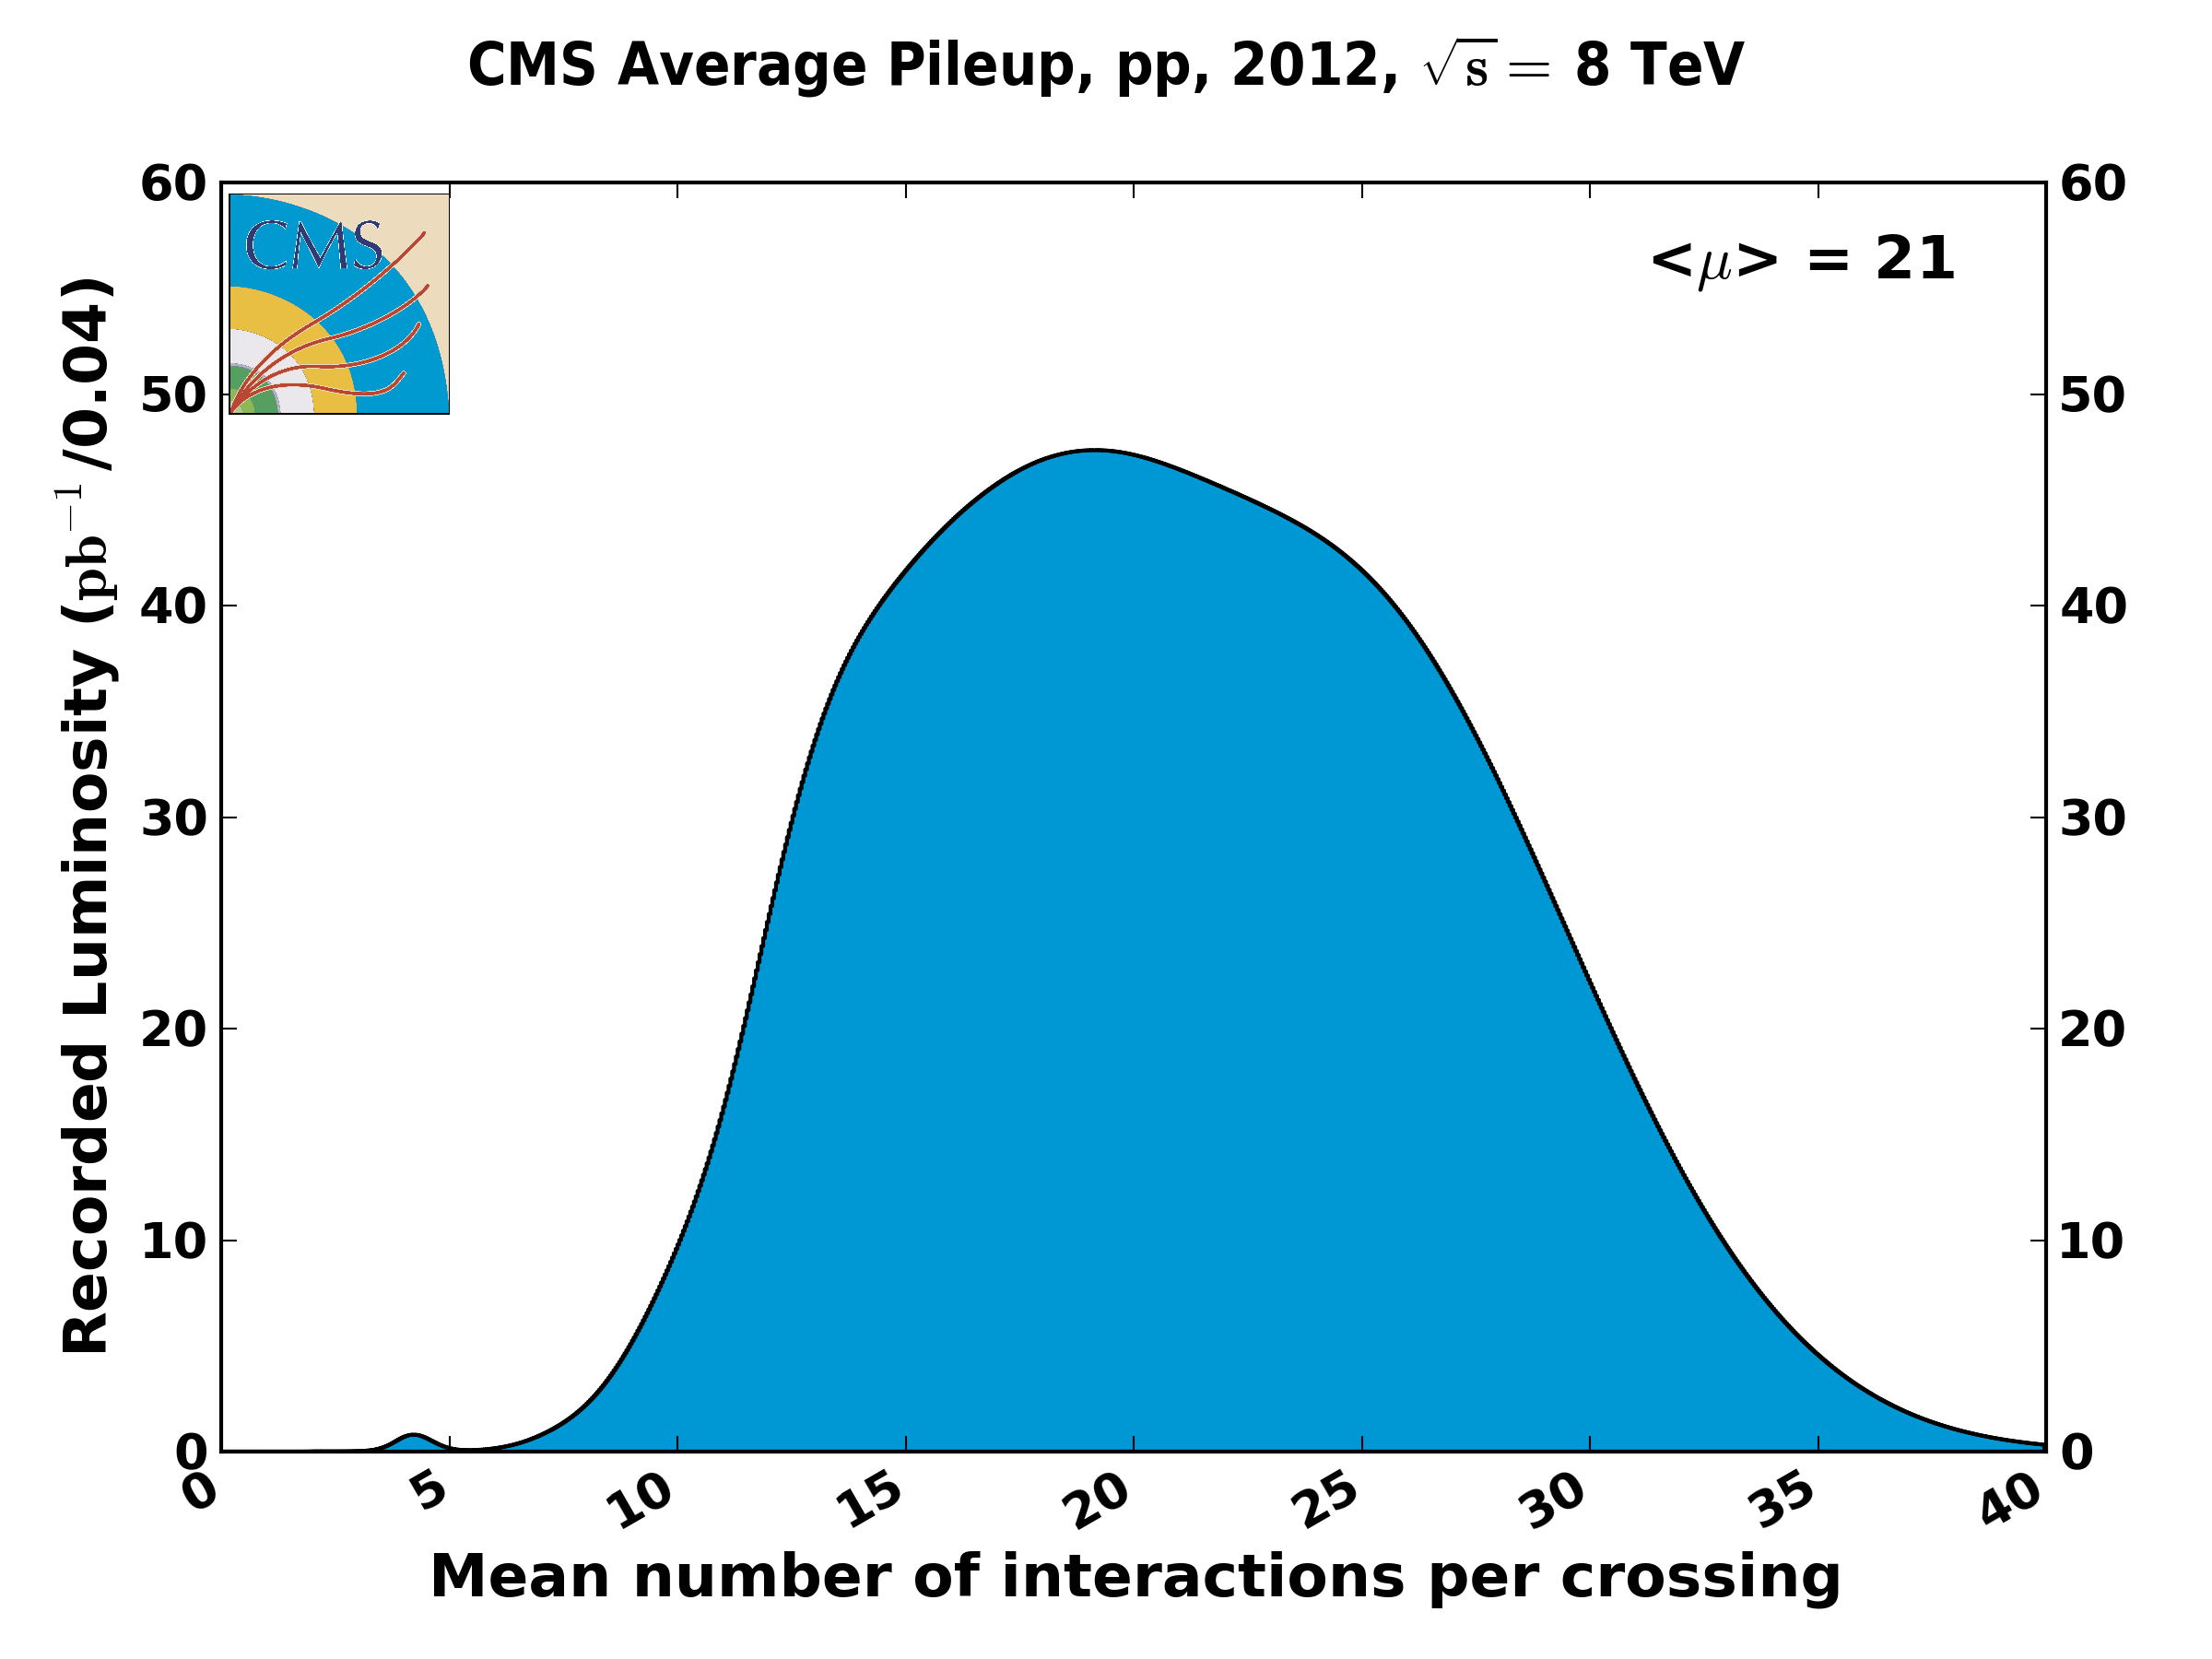
\includegraphics[width=0.7\textwidth]{LHC/pileup.png}
	\captionof{figure}{Distribution du nombre de collisions par croisement de faisceaux.}
	\label{pile-up}	
\end{minipagewithmarginpars}

\subsection{Vers le High-Luminosity LHC (HL-LHC)}
De par l'envergure de la machine, du nombre d'expériences nécessitant le bon fonctionnement du LHC et le nombre de personnes impliqués dans ce projet, celui-ci à fait l'object d'un calendrier prévisionnel (cf.fig\ref{roadmap}). Ce calendrier est diviser en deux grande période: la \textbf{Phase I} (2010-2023) et la  \textbf{Phase II} (2023-2035). Chaque phase est elle-même divisée en plusieurs périodes comportant des arrêts techniques et des arrêt beaucoup plus long appellé "Long Shut-down (LS)". Ces arrêts permettent d'améliorer le LHC ainsi que d'avoir accés au détecteurs à des fins de maintenance et d'améliorations. L'arrêt le plus important à venir est le LS3. Il est censé durer une trentaine de mois et permettre la mise à niveau du LHC vers le HL-LH.

\begin{minipagewithmarginpars}[h]{0.95\textwidth}
	\centering
	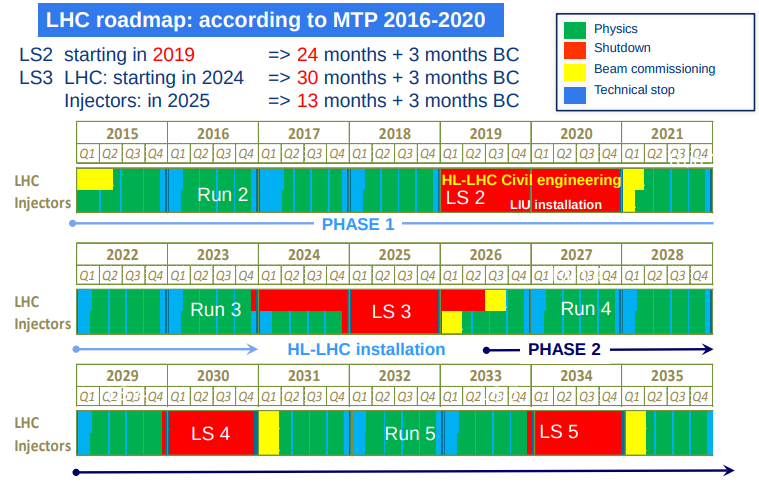
\includegraphics[width=0.9\textwidth]{LHC/roadmap.png}
	\captionof{figure}{Calendrier prévisionnel du LHC.}
	\label{roadmap}	
\end{minipagewithmarginpars}

\subsubsection{Le HL-LHC}
La mise à niveau du LHC en HL-LHC vis à multiplier la luminosité par 10 par rapport à la luminosité nominale du LHC.

Le but est de produire environ 140 événement de pile-up par croisement de faisceau contre une trentaite actuellement. Pour cela le faisceau devra être plus intense et plus concentré qu'actuellement.Afin d'y parvenir de nombreux paramètres du collisionneur et de la chaine d'accélération vont être mis à niveau (cf.fig\ref{man}).

\begin{itemize}[label=$\bullet$]
	
 \item Un nouveau système optique est à l'étude afin d'adapter la concentration du faisceau au cours du temps afin de maintenir une luminosité constante tout le long de la durée de vie du faisceau. D'autre instrument de mesures des paramètres des faisceaux seront également installés.
 
 \item Des aimants de 12T contre 8T pour le présent système seront installé à l'avant de ATLAS et CMS afin de mieux collimer les faisceaux.
 
 \item Des cavités supraconductrices vont être installé en vue d'orienté les paquets de particules en leur donnant un moment transverse afin d'augmenter la section efficace. Cette configuration est appellé configuration en "crabe".
 
 \item L'accroissement du nombre de particule nécessite un renforcement des protections afin de ne pas abimer la machine. 60 des 118 collimateurs qui permettent l'absorptions de particules qui s'échappent de la trajectoire nominale du faisceaux seront remplacés et 15 à 20 nouveaux seront installés.
 
 \item Afin d'insérer ces nouveaux collimateurs, quatre des dipoles de 15 mètres de long seront remplacés par quatre paires d'aimants beaucoups plus puissant. Il seront capable de produire un champ magnetique de 11T contr 8.3T pour les aimants actuels
 
 \item Deux nouvelles caverne de service de 300 mètres de long vont être creusés prêt des expérience CMS et ATLAS. Elles abriteront les services nécessaires à ces expériences et ceux sensible aux radiactions (convertisseur de courant, cryogénie etc.)
 
 \item De nouvelles lignes de transmitions electrique vont également être iinstallé. Ces cables seront fait d'un matériaux superconducteur ( diboride de magnésium) capable de fonctionner à haute température (20K) et beaucoup plus stable que les supraconducteur conventionnels. Il permettront de porter des courants de plus de 100 000 A.
 \item La chaine d'accélération sera elle aussi mise à niveau. Dés 2020, un nouveau Accélérateur linéaire appellé LINAC4 (cf.fig\ref{linac4}) va remplacer le LINAC2. Les trois autres accélerateur de la chaine (PSB, PS ET SPS ) auront également droit à de améliorations.
\end{itemize}

\marginpar
{
	
	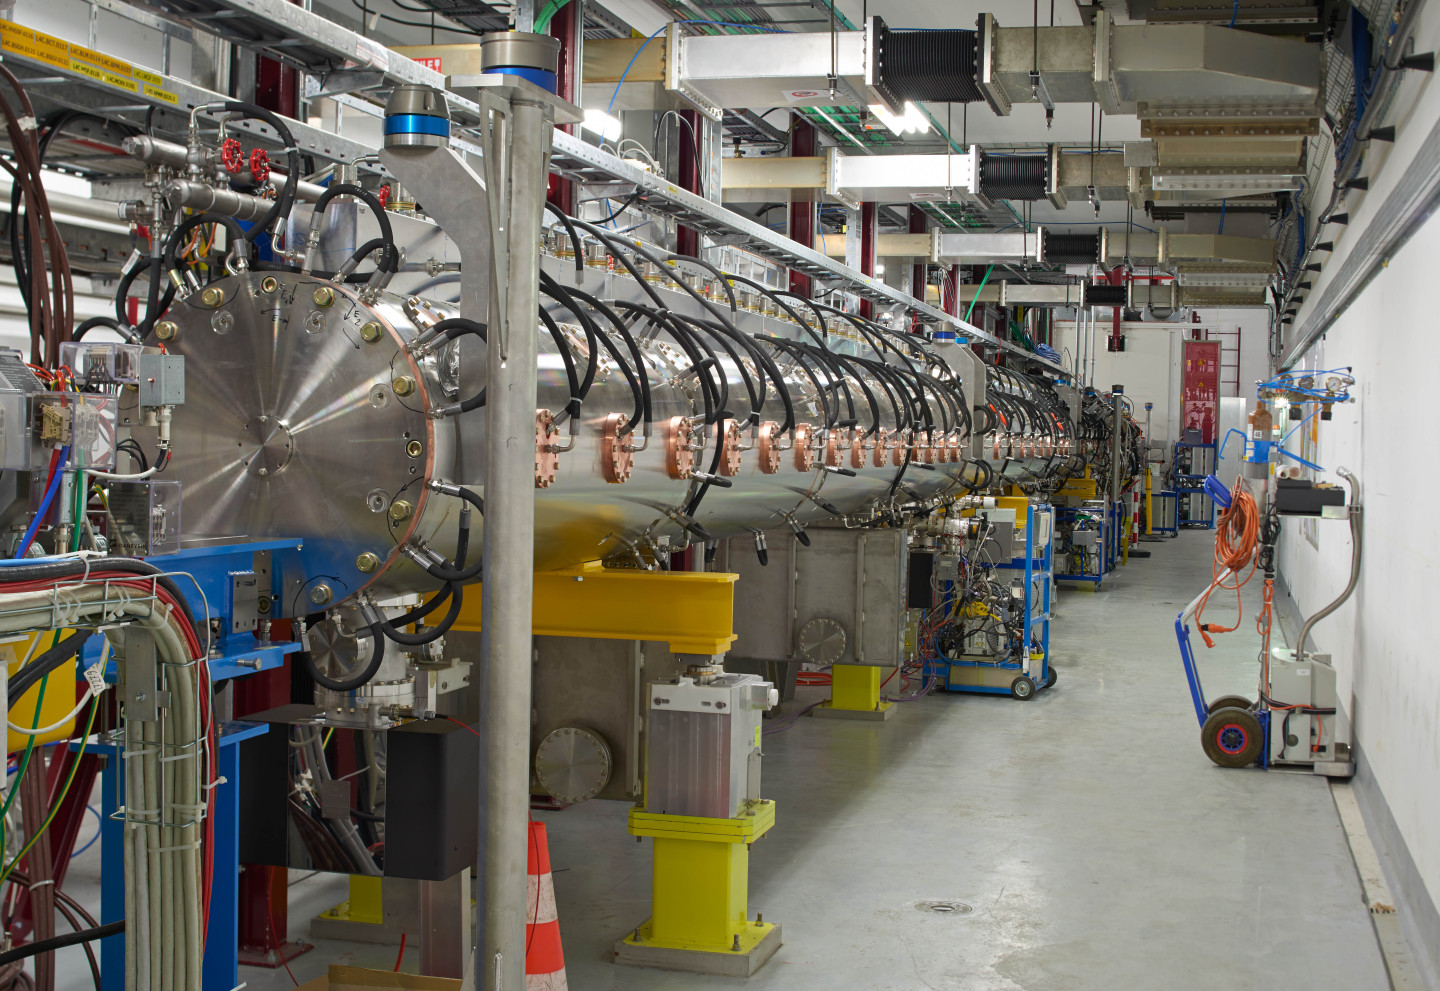
\includegraphics[width=\marginparwidth]{LHC/linac4.jpg}
	\captionof{figure}{Photo du LINAC4.}
	\label{linac4}
}
\begin{minipagewithmarginpars}[h]{0.95\textwidth}
	\centering
	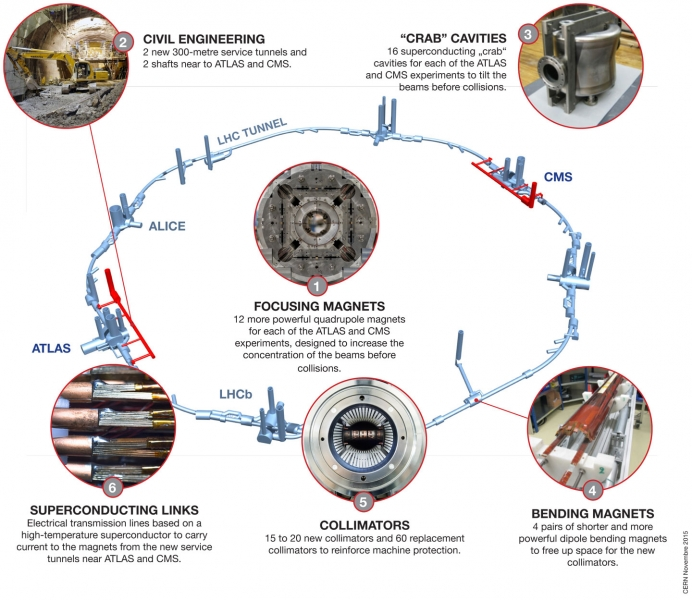
\includegraphics[width=0.95\textwidth]{LHC/man.jpg}
	\captionof{figure}{Schame montrant les différents types de mise à niveau nécessaire au HL-LHC.}
	\label{man}	
\end{minipagewithmarginpars}

Le tableau \ref{comparaison} donne les différents paramètres selon plusieurs configurations envisagés par rapport au paramètres nominaux actuels du LHC

\begin{table}
\tiny
\centering
\begin{tabular}{|S{P{62mm}}|S{P{15mm}}|S{P{15mm}}|S{P{15mm}}|S{P{15mm}}|}
	\hline 
	Paramètre &\shortstack{LHC Nominal \\ (design report)}&\shortstack{HL-LHC 25ns \\ (standard)}&\shortstack{HL-LHC 25ns \\ (BCMS)}&\shortstack{HL-LHC \\ 8b+4e$^{12}$}\\ 
	\hline 
	\shortstack{ du faisceau [TeV]} & \shortstack{7} & \shortstack{7} & \shortstack{7} & \shortstack{7} \\ 
	\hline 
	\shortstack{Nombre de proton par paquet $N_{b}$}&\shortstack{$1.15\times 10^{11}$}&\shortstack{$2.2\times 10^{11}$}& \shortstack{$2.2\times 10^{11}$}&\shortstack{$2.3\times 10^{11}$}\\ 
	\hline 
	Nombres de paquets $n_{b}$& 2808 & 2748 & 2604 & 1968 \\ 
	\hline 
	\shortstack{Nombre de collisons aux point P1 et P5}& 2808 & 2736 & 2592 & 1960 \\ 
	\hline 
	Courant du faisceau [A]& 0.58 & 1.09 & 1.03 & 0.82 \\ 
	\hline 
	angle x-ing [$\mu$ rad] & 285 & 590 & 590 & 554 \\ 
	\hline 
	$\beta{*}$ [m]& 0.55  & 0.15 & 0.15 & 0.15 \\ 
	\hline 
	$\epsilon_{n}$ [$\mu$ m]& 3.75 & 2.50 & 2.50 & 2.20 \\ 
	\hline 
	$\epsilon_{l} [eVS]$& 2.50 & 2.50 & 2.50 & 2.50 \\ 
	\hline 
	r.m.s. de la longueur du paquet [m]& $7.55\times 10^{-2}$  & $7.55\times 10^{-2}$ & $7.55\times 10^{-2}$ & $7.55\times 10^{-2}$ \\ 
	\hline 
	paramètre de Piwinski & 0.65 & 3.14 & 3.14 & 3.14 \\ 
	\hline 
	\shortstack{Facteur de perte total $R0$ sans cavité "crabes"}& 0.836 & 0.305 & 0.305 & 0.304 \\ 
	\hline 
	\shortstack{Facteur de perte total $R1$ avec cavité "crabes"}& (0.981) & 0.829 & 0.829 & 0.828 \\ 
	\hline 
	\shortstack{Pic de luminosité sans cavité de type "crabe" [cm$^{-2}$s$^{-1}$]}& $1.00\times 10^{34}$ & $7.18\times 10^{34}$ &$6.80\times 10^{34}$ & $6.38\times 10^{34}$ \\ 
	\hline 
	\shortstack{Luminosité virtuelle avec cavité de type "crabe" \\$L_{peak}R_{1}/R_{0}$[cm$^{-2}$s$^{-1}$] } & $1.18\times 10^{34}$ & $19.54\times 10^{34}$ & $18.52\times 10^{34}$ & $17.40\times 10^{34}$ \\ 
	\hline 
	\shortstack{ Événements / croisement de faisceaux sans nivellement \\et sans cavités de type "crabe"}& 27 & 198 & 198 & 246 \\ 
	\hline 
	Luminosité nivellé [cm$^{-2}$s$^{-1}$]& - & $5.00\times 10^{34}$ &  $5.00\times 10^{34}$& $3.63\times 10^{34}$ \\ 
	\hline 
	\shortstack{Événements/croisement de faisceaux avec nivellement \\ et cavités de type "crabe" pour HL-LHC}& 27 & 138 & 146 & 140 \\ 
	\hline 
	\shortstack{Pic de densité linéaire d'événement pile-up [evt/mm] \\(maximum pour des faisceaux stables)%Pic de densité linéaire d'événement pile-up \\ [événements/mm] (maximum pour des faisceaux stables)
	} & \shortstack{0.21} & \shortstack{1.25} & \shortstack{1.31} & \shortstack{1.28} \\ 
	\hline 
	\shortstack{temps de nivellement [h]\\ (aucune augmentation d'émittance)}& - & 8.3 & 7.6 & 9.5 \\ 
	\hline 
	$N_{b}$ à l'injection dans le LHC& $1.20\times 10^{11}$ & $2.30\times 10^{11}$ & $2.30\times 10^{11}$ &$2.40\times 10^{11}$  \\ 
	\hline 
	$n_{b}$ par injection& 288 & 288 & 288 & 224 \\ 
	\hline 
	$\epsilon_{n}$ à l'extraction du SPS& 3.40 & 2.0 & <2.00 & 1.70 \\ 
	\hline 
\end{tabular} 
\caption{List des principaux paramètres du faisceau du HL-LHC. La colonne intitulé "standard" est le design pris comme objectif, les deux autres colonnes reprèsentent des variantes de ce design. Pour comparaison, les paramètres du faisceau du LHC dans son design nominal est reporté dans la première colonne.}
\label{comparaison}
\end{table}

L'augmentation de la luminosité va amener à la mise à niveau des détecteurs et notamment CMS afin de supporter le nombres importants de collisions par croisements de faisceaux. D'autres améliorations et travaux de maintenance seront également réalisé durant cette arrêt. 